\chapter{An Automated Method for LAT Analysis of the Galactic Supernova Remnant Population}\label{chap:snrcat}


\section{Introduction}\label{snrCat:Intro}
Two of the primary science goals of the \lat{}  are to 1. resolve the \gam~sky, uncovering the nature of the unidentified sources detected by \egret{}, and 2. to understand the mechanisms of cosmic particle acceleration \citep{atwood09}. In this chapter, we describe our efforts towards addressing these questions by studying the \gam{} emission coincident with sources comprising the population of known radio emitting \snrs{}.

Prior to this work, several individual studies with the \lat{} had successfully resolved spatially extended emission from \snrs{} \citep[and references therein]{2FGL}, yet no systematic analysis leveraging the \lat{}'s full-sky coverage had thus been attempted. We performed for the first time a uniform study of the \snrs{} in aggregate to measure the properties common to these objects. An understanding of these common characteristics allows us to assess \snrs{} as a class of \gam{} and \cray{} emitting objects and serves as the impetus for this uniform analysis of the known Galactic \snrs{}. We report here on the published results from the \snrcat{} \citep{snrCat}.
 

%%%%%%%%%%%%%%%%%%%%%%
%%%%%%%%%%%%%%%%%%%%%%

\section{The \ptlike{} Maximum-Likelihood Package and \srcs{}}\label{snrcat:ptlk}

As described in Chapter \ref{FGST:analysis}, maximum-likelihood analysis is the ideal method for determining the properties of \lat{}-observed sources due to the ``counting-experiment" nature of \FermiLat{}. The standard maximum-likelihood tools for analyzing \lat{} data are implemented via the \Fermi{} Science Tools, and in particular \gtlike{}.  Despite being the optimum method, likelihood analysis of \lat{} data is complex due to the highly non-linear performance of the instrument and can be computationally expensive. It is necessary to manage the data and response of the telescope as well as the source and background models. Furthermore, due to the broadening of the \psf{} at low energies, even when studying a single source, it is necessary to include in the model descriptions of multiple surrounding sources. The \ptlike{} binned maximum likelihood package was created to ameliorate some of these issues. Described in detail in \cite{Kerr10}, \ptlike{} is an alternate likelihood analysis framework (a collection of Python modules with additional wrappers for accessing C++ code), designed to be interactive and rapidly evaluate likelihoods.  

There are several ways in which \ptlike{} improves in efficiency compared to the Science Tools. It saves computational time, while sacrificing some accuracy,
with several assumptions and approximations, such as the \psf{} not varying strongly with photon incidence angle (allowing a single \psf{} for each individual bin), and sources having a steady flux in individual short time bins. Most importantly though, \ptlike{} varies the size of spatially binned \heal{} pixels \citep{Gorski05} according to energy. The \psf{} at lower energies is large and each energy bin can contain multiple counts, while at higher energies, the \psf{} shrinks and many pixels will not contain even a single count. \ptlike{} creates \heal{} bins that are approximately the size of the \psf{} at a given energy, and disregards empty bins to speed up the likelihood calculation.

In addition to these computational, time saving efficiencies, tools to analyze spatially extended sources have also been built into the \ptlike{} framework. Studying the position and extension of an extended source, while possible with the standard \Fermi{} Science Tools, is a cumbersome process. \gtlike{} is not capable of simultaneously maximizing the likelihood of a source's spectral and spatial parameters, so to assess the morphology of a source, an iterative process of fitting a spatially fixed source's spectrum and then varying the sources centroid and extension is required. To address the issues that arise when studying individual extended sources, \cite{Lande12} developed and validated spatial likelihood fitting tools for \ptlike{}, taking advantage of the time-saving properties built therein.

To fit the position and extension of a source, \ptlike{} assumes that the spatial and spectral distribution of a source's expected photon distribution are separable. The extended source's shape is convolved with the \lat{} \psf{} (which is a function of energy) to determine the expected distribution. Then, the {\tt minuit} numerical minimization library\citep{James75} is used to maximize the likelihood of the model by simultaneously varying the spectrum, extension, and position of the source. Various geometric surface brightness models are built into \ptlike{}, including, but not limited to a uniform intensity disk and ring, and a 2D Gaussian, with radially and non-radially symmetric versions of each. Akin to the speed optimizations mentioned previously, for radially symmetric sources, \ptlike{} calculates the angular integral of a source's expected photon distributions analytically to save computational time.

The significance of extension of a source is determined by using the \lrt{}, described in Chapter \ref{FGST:analysis}. Applying the \lrt{} to the hypothesis of a spatially extended source, we can calculate the significance of a source being extended compared to that of the source being modeled as point source as:

\begin{equation}\label{eq:tsext}
\rm \ts{}_{ext} \equiv 2\log(\like_{\rm es}~/ \like_{\rm ps}) = \ts{}_{es} - \ts{}_{ps},
\end{equation}

\cite{Lande12}, extended (and verified) the definition of \ts{} (see equation \ref{eq:LRT}) to calculating the significance of extension, replacing the source flux with its radius. The uncertainty of the extension parameter is estimated by fixing a source's position while varying the extension until the log likelihood decreases by 1/2 from the maximum value (\ie{}  1$\sigma$ errors).  \jamie{use that TS vs extension figure I didn't include in the G150 paper to demonstrate where the TS drops by half from the peak?} A similar procedure is used to estimate the errors on a source's position, but rather,  fixing the extension and spectrum \citep{2FGL}. While \ptlike{} is the tool we used for the analyses described above, \gtlike{} is the standard likelihood tool for estimating the best-fit spectral parameters since it is expected to be slightly more accurate than \ptlike{} due to the approximations \ptlike{} makes (described above). For the studies in this thesis, we used \ptlike{} to calculate extension and source positions, and then use the \ptlike{} results as a starting point for the likelihood parameter estimation of spectra with \gtlike{}.

With its efficient likelihood calculations, and ability to simultaneously fit both the spectral and spatial parameters of a source, \ptlike{} is ideally suited for large-scale studies (like the all-sky analyses performed for the \lat{} point source catalogs), and analyses requiring several iterations. Studying the \gam{} emission from the population of Galactic \snrs{} is precisely the sort of analysis that \ptlike{} was designed to perform. To attain the best understanding of a source of interest, the best characterization of the corresponding \roi{} is necessary. In particular, to understand the \gev{} emission from a potentially extended \snr{}, it is important to quantify the surrounding emission because of the steep energy-dependence of the \lat{} \psf{}. This can be especially challenging in dense source and strong diffuse-dominated regions, like the Galactic plane where the \snrs{} we are studying lie. We have developed an automated method for systematically locating and modeling all potential point and/or extended sources in an \roi{} using \ptlike{}. 

A typical \lat{} analysis starts by including all sources from the most recent \lat{} point source catalog and modifying the \roi{} to suit ones needs. Unmodeled emission can arise if using a dataset longer than that used in the most recent catalog or by focusing on a different energy range compared to that of the catalogs. We created a Python subclass of the primary \ptlike{} analysis object (which works within that framework, inheriting all of the class' features, while adding new functionality) to systematically and uniformly characterize sources in an \roi{} by finding residual, unmodeled emission in the region and iteratively add sources to the \roi{} to account for this emission. The main module in the designed codebase was dubbed \srcs{}. 

The general work flow of \srcs{} is to start with a model of the \roi{}, including some combination of the diffuse background components, point  and extended sources. \srcs{} reads in a residual \ts{} map or creates one on the fly if none is passed in. Residual emission is detected by finding the peak emission in the \ts{} map and adding a source to the existing \roi{} at the position of the peak pixel. Either all point or extended sources can be iteratively detected and added to the \roi{}. For the \snrcat{}, we exclusively ran \srcs{} in point source mode. Chapter \ref{chap:2FHL} provides an application of \srcs{} for extended sources. 

In point source mode, a point source with a \pl{} spectrum is added to the model of the region, a likelihood fit of the \roi{} is performed, and subsequently, the source's position is localized. Similarly, in extended mode a \pl{} extended source (of any morphological form included in \ptlike{}) is added to the \roi{} with a small seed radius, and the spatial parameters of the newly added source are fit simultaneously with the spectra of the other sources already in the model. If the source has ${\rm TS_{ext} < 16}$ (equivalent to a  4$\sigma$ extension significance and validated through simulations in \cite{Lande12} as a reasonable extension detection significance), the extended source is replaced with a point source and the iteration continues as in point source mode. To extend the functionality of \srcs{} and make it generally applicable to a multitude of \lat{} analyses, several optional methods were built in. 

One such option is to test the newly added source for signs of spectral curvature (described further in Chapter \ref{snrcat:AddSrcs}). If the source is found to show significant spectral curvature, the appropriate curved spectral model is retained, otherwise, we revert to the best-fit \pl{} model. Another option provided is to fix the new sources spectrum if it is within a given angular separation of the center of the RoI to limit the number of free parameters for the likelihood fit and aid in proper convergence. If the source of interest being studied is not central in the \roi{} it might be beneficial to free the spectral parameters of sources within a given distance of the newly added source rather than from the center of the \roi{}. This choice was also built into \srcs{}. Further, we included an option to refit the extension of any extended source already in the model at each iteration if they are within a given distance of the new (point or extended) source. Due to the broad size of the \psf{}, nearby source spectra can be influenced by each other, (particularly for extended sources) so the iterative procedure allows the likelihood to relax to a preferred value when adding new sources.

Throughout the \srcs{} process, various checks are performed to ensure that parameter values are reasonable,
the likelihood fit converges, and the procedure is generally running as expected. The range of permissible fit values for a parameter can be limited, the values of the parameters themselves can be fixed, or a consistently poorly-fit source can be automatically removed from the model. During the source localization step, if the fit goes awry and the source wanders too far from its initial position, the position of the source can be rolled back to its staring location and fixed. Checks were also included to keep track of the Galactic diffuse and isotropic emission models to ensure they were adequately fit.

The penultimate step of the iteration is to produce various diagnostic plots and output information about the fits, the spectral and spatial parameters of each source in the model, and other relevant information such as the \ts{} of the source and loglikelihood of the fit. Finally, a new residual \ts{} map of the region is created and the source addition procedure repeats until a given threshold in \ts{} is reached. The peak pixel \ts{} found in the residual \ts{} map does not necessarily decrease monotonically, as is expected of the actual \ts{} of successive sources as more of the emission is accounted for and the model improved. Since the peak pixel TS can fluctuate a bit, to ensure that we do not miss significant sources in the \roi{}, we continue adding sources until the \ts{} threshold is reached for some number of successive sources (discussed further in \ref{snrcat:AddSrcs}). After sources are no longer being added to the region, we iteratively remove sources with \ts{} less than a given threshold (typically ${\rm TS < 16}$, again see Chapter \ref{snrcat:AddSrcs}) starting with the lowest \ts{} sources first. As each source is removed, we refit the \roi{}, including any extended sources close to the removed source. When the TS of all sources in the \roi{} are above threshold, we deem the emission in the \roi{} to be sufficiently characterized.  

In the following sections, we detail the application of \srcs{} to studying the \gev{} Galactic \snr{} population and describe the analysis and results presented in \cite{snrCat}. 

%The peak pixel \ts{} value determined from the \ts{} map and used as the seed position for a newly added source is not the same as the \ts{} of the source itself. The peak pixel does not necessarily decrease monotonically, as is expected of the \ts{} of successive sources as more of the emission is accounted for and the model improved We can see how they differ by recalling that a \ts{} map is created by placing a point source at each grid location in the map and finding the \ts{} of the source at that specific pixel. While the \ts{} of the source itself (log likelihood ratio of the hypothesis with the source and without) is determined 

%%%%%%%%%%%%%%%
%%%%%%%%%%%%%%%

\section{Galactic Supernova Remnants}\label{sncat:SNRSelection}
In this work we focus on the 279 currently known Galactic SNRs. They are derived from the $274$~SNRs noted in the catalog of \citet[hereafter Green's catalog]{Green09}, plus five additional SNRs identified following its publication. 
All but $16$ of these SNRs have been identified by their radio synchrotron emission, so their centroids and extensions are primarily determined from the radio. When the radio detection is not securely identified through the synchrotron emission, positional information is obtained from the optical, X-ray, or TeV observations that identified the SNR, as noted in Green's catalog. The catalog is thought to be complete down to a $1$\,GHz radio surface brightness limit of $\approx 10^{-20}$\,W\,m$^{-2}$\,Hz$^{-1}$\,sr$^{-1}$ (i.e.\,$1$\,MJy\,sr$^{-1}$). However, selection effects are known to bias radio surveys against the identification of radio faint and small angular size remnants \citep{Green04,Brogan06}. We note that as this work neared completion, a revised catalog of $294$~SNRs was published \citep{Green14}, representing only a small increase ($<10\%$) over the previous catalog.


%%%%%%%%%%%%
%%%%%%%%%%%%

\section{Analysis Methods}\label{snrcat:AnalysisMethod}
To systematically analyze the \FermiLat{} \gam{} data, we apply a maximum likelihood \citep{mattox96} framework to \rois{} centered on known SNRs \citep{Green09}. For each SNR, we begin by constructing a model for the spectral and spatial dependence of the \gam{} emission which includes significant point sources in the RoI. We then test for the existence of a \gam{} source near the center. This includes determining the most likely position and extension of the candidate source and testing for spectral curvature, rather than assuming it follows a \pl{} across the energy range studied. In cases where we find no significant source associated with the SNR, we calculate upper limits on the flux. We calculate both statistical and systematic errors, where the latter are estimated from both the uncertainty in the effective area and the effects of changing the \iem{}, which accounts for \gam{}s produced by CR interactions with interstellar gas and radiation fields in the Milky Way. 

This analysis uses both the standard Science Tools (version 09-32-05), including \gtlike{}, and the \ptlike{} analysis package~\citep{Kerr10} which has been developed and verified for characterizing source extension for \FermiLat{} data \citep{Lande12}. $\S$\ref{snrcat:Data} describes our data selection; $\S$\ref{snrcat:AddSrcs} details our new method for automatically finding point sources in the \FermiLat{} \g-ray emission; and $\S$\ref{snrcat:DetectMethod} discusses the detection method.

\section{Data Selection}\label{snrcat:Data}
This catalog was constructed using 3 years of LAT survey data from the Pass~$7$~(P7) ``Source'' class and the associated P7V6 \irf{}.This interval spans $36$\,months, from $2008$\,August\,$4$ to $2011$\,August\,$4$ (mission elapsed time $239557417-334108806$). The Source event class is optimized for the analysis of persistent LAT sources, and balances effective area against suppression of background from residual misclassified charged particles. We selected only events within a maximum zenith angle of $100$\degr{} and use the recommended filter string ``DATA\_QUAL==1 \&\& LAT\_CONFIG==1'' in {\tt gtmktime}\footnote{See LAT data selection recommendations at: \url{http://fermi.gsfc.nasa.gov/ssc/data/analysis/documentation/Cicerone/Cicerone_Data_Exploration/Data_preparation.html}.}. 
The P7 data and associated products are comparable to  those used in the other \gam{} catalogs employed in this work. We used the first three years of science data for which the associated IEM is suitable for measuring sources with extensions $>2$\degr \footnote{See the LAT caveats, \url{http://fermi.gsfc.nasa.gov/ssc/data/analysis/LAT_caveats.html}, particularly those for the IEM developed for Pass~$7$ reprocessed data described in \url{http://fermi.gsfc.nasa.gov/ssc/data/access/lat/Model_details/FSSC_model_diffus_reprocessed_v12.pdf}.}. A detailed discussion of the instrument and event classes can be found in \cite{atwood09} and at the \Fermi{} Science Support Center\footnotemark[1].

For each of the 279 SNRs we modeled emission within a $10$\degr{}\,radius of the SNR's center. As a compromise between number of photons collected, spatial resolution, and the impact of the \iem{}, we chose $1$\,GeV as our minimum energy threshold. The limited statistics in source class above $100$\,GeV motivated using this as our upper energy limit. 

To avoid times during which transient sources near SNRs were flaring, we removed periods with significant weekly variability detected by the \Fermi{} All-sky Variability Analysis (FAVA) \citep{fava13}. We conservatively defined a radius within which a flaring source may significantly affect the flux of a source at the center. We take this distance to be the radio radius of an SNR plus $2.8$\degr, corresponding to the overall $95\%$~containment radius for the \FermiLat{} point spread function (PSF) for a $1$\,GeV photon at normal incidence \citep{lat_perf}. The time ranges of FAVA flares within this distance were removed in $23$~RoIs, leaving $\geq 98.9\%$ of the total data in each RoI.

%%%%%%%%%%%%%%%%%%
%%%%%%%%%%%%%%%%%%
\section{Input Source Model Construction}\label{snrcat:AddSrcs}
To characterize each candidate SNR we constructed a model of \gam{} emission in the RoI which includes all significant sources of emission as well as the residual background from CRs misclassified as \gam{}s. We implemented an analysis method, built upon the \srcs{} method described in \ref{snrcat:ptlk}, to create and optimize the 279 models for each of the $279$~RoIs. For each RoI, we initially included all sources within the $10$\degr{} RoI listed in the \twofgl{} \citep{2FGL}, based on $2$\,years of Source class data. To this we added pulsars from the \twopc{} \citep{2PC}, based on $3$\,years of source class data, with 2PC taking precedence for sources that exist in both. 
For the diffuse emission we combined the standard \iem{} corresponding to our P7 data set, gal\_2yearp7v6\_v0.fits, with the standard model for isotropic emission, which accounts for extragalactic diffuse \gam{} emission and residual charged particles misclassified as \gam{}s. Both the corresponding isotropic model, iso\_p7v6source.txt, and the IEM are the same as used for the 2FGL catalog analysis\footnote{Further details on the diffuse emission models are available at \url{http://fermi.gsfc.nasa.gov/ssc/data/access/lat/BackgroundModels.html} \jamie{and in Chapter blah]}}. 

Compared to 2FGL, we used an additional year of data and limited the energy range to $1-100$\,GeV. This can result in different detection significances and localizations than previously reported in 2FGL. To account for these effects, we recreated the RoIs' inner $3$\degr{}\,radius regions, which encompass the radio extents of all known SNRs, observed to be $\leq 2.6$\degr{} and allows a margin for the LAT PSF. The weighted average $68\%$~containment radius of the LAT PSF for events at $1$\,GeV is $\sim0.7$\degr{} \citep{lat_perf}. We note that this implicitly assumes that an SNR's GeV extent should not be more than about an order of magnitude larger than its radio extension and also note that the selection biases stated in Green's catalog limit the range of known SNRs' radio extensions. 

To build the inner $3$\degr{}\,radius model of each RoI, we first removed all sources except identified \agn{} and pulsars, whose positions on the sky are independently confirmed by precise timing measurements \citep{2PC}. Retained AGN were assigned their 2FGL positions and spectral model forms. Pulsars' positions and spectral forms were taken from 2PC. 2FGL sources identified or associated with SNRs are removed when they lie within the inner $3$\degr{}. 

Using \srcs{}, we generated a \ts{} map via \ptlike{} on a square grid with $0.1$\degr{}\,$\times$\,$0.1$\degr{} spacing that covers the entire RoI. At the position of the maximum TS value, we added a new point source with a Power Law (PL) spectral model:
\begin{equation}
\label{eqn:PL}
\frac{dN}{dE} = N\frac{(-\Gamma+1)E^{-\Gamma}} {E_{\rm max}^{-\Gamma+1} - E_{\rm min}^{-\Gamma+1}}
\end{equation}
where $N$ is the integrated photon flux, $\Gamma$ is the photon index, and $E_{\rm min}$ and $E_{\rm max}$ are the lower and upper limit of the energy range in the fit, set to $1$\,GeV and $100$\,GeV, respectively.
We then performed a maximum likelihood fit of the RoI to determine $N$ and $\Gamma$ and localized the newly added source. 
The significance of a point source with a PL spectral model is determined by the $\chi^2_n$ distribution for $n$ additional degrees of freedom for the additional point source, which is typically slightly less than~$\sqrt{\textrm{TS}}$

To promote consistent convergence of the likelihood fit, we limited the number of free parameters in the model. For sources remaining after the removal step, described above, we freed the normalization parameters for the sources within $5$\degr{} of the RoI center, including identified AGN and pulsars. For 2FGL sources between $5$\degr{} and $10$\degr{}, we fixed all parameters. The spectrum of the IEM was scaled with a PL whose normalization and index were free, as done in 2FGL. For the isotropic emission model, we left the normalization fixed to the global fit value since the RoIs are too small to allow fitting the isotropic and Galactic IEM components independently. The isotropic component's contribution to the total flux is small compared to the IEM's at low Galactic latitudes.

After localizing them, the new sources were tested for spectral curvature. In each of the four~energy bands between $1$ and $100$ GeV, centered at $1.8$, $5.6$, $17.8$ and $56.2$\,GeV, we calculated the TS value for a PL with spectral index fixed to $2$ and then summed the TS values. We refer to this as $\mathrm{TS_{band fits}}$. A value for $\mathrm{TS_{band fits}}$ much greater than the TS calculated with a PL ($\mathrm{TS_{PL}}$) suggests that, with a more rapid calculation, that the PL model may not accurately describe the source. Analogously to 2FGL, we allow for deviations of source spectra from a PL form by modeling sources with a log-normal model known colloquially as LogParabola or logP:
\begin{equation}
\newcommand{\pfrac}[2]{\left(\frac{#1}{#2}\right)} \frac{dN}{dE} = N_0\pfrac{E}{E_b}^{-(\alpha + \beta\log(E/E_b))}
\label{eqn:logP}
\end{equation}
where $N_0$ is the normalization in units of photons/MeV, $\alpha$ and $\beta$ define the curved spectrum, and $E_b$ is fixed to $2$\,GeV\footnote{Note: $E_b$ is a scale parameter which should be set near the lower energy range of the spectrum being fit and is usually fixed, see \citet{massaro04}}. If $\mathrm{TS_{band fits} - TS_{PL}} \geq 25$, we replaced the PL spectral model with a logP model and refit the RoI, including a new localization step for the source. We retained the logP model for the source if the global log likelihood across the full band improved sufficiently: 
$\mathrm{TS_{curve}} \equiv 2 ($\logL{}$_{\mathrm{logP}}-$\logL{}$_{\mathrm{PL}}) \geq 16$. 
Otherwise we returned the source to the PL model which provided the better global log likelihood. Across all RoIs, less than $2\%$ of the newly added sources retained the logP model. 

We continued iteratively generating TS maps and adding sources within the entire RoI until additional new sources did not significantly change the global likelihood of the fit. The threshold criterion was defined as obtaining $\mathrm{TS < 16}$ for three consecutively added new sources, denoted as $\mathrm{N_{TS < 16} = 3}$. Despite iteratively adding a source at the location of the peak position in the TS map, the TS values of new sources may not decrease monotonically with iteration for several reasons. First, source positions were localized after fitting the RoI and generating the TS map. Second, some added sources were fit with a more complex spectral model than a simple PL. Finally, when creating the TS map, we fixed the source's spectral index to $2$, whereas when adding the actual source to the model, we allowed its index to vary. Figure \ref{fig:flowChart} shows a flow chart encapsulating the \srcs{} method applied to the \snrcat{} described above.

\begin{figure}[ht!]
	\centering
	\makebox[\linewidth]{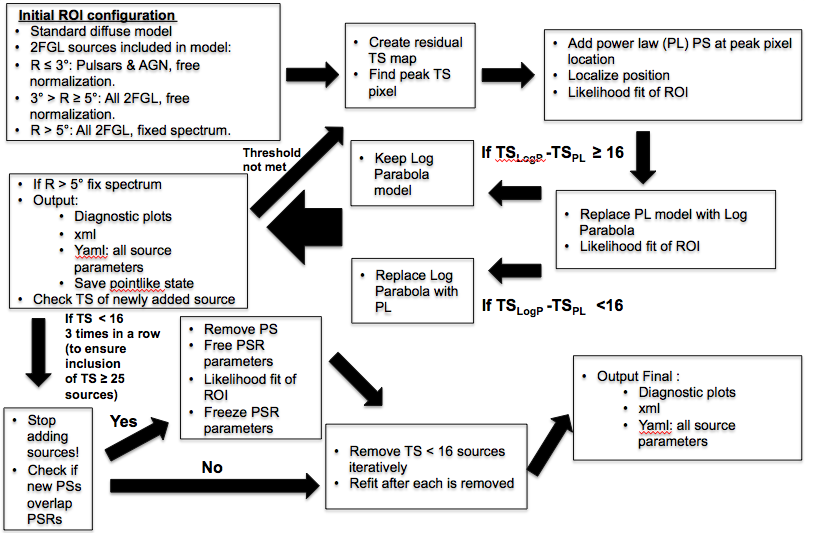
\includegraphics[width=1.0\columnwidth]{Figures/addSrcs_snrCat_FlowChart.png}}
	\caption[\srcs{} Flow chart]{Flow chart of the \srcs{} application for the \snrcat{}}
	\label{fig:flowChart}
\end{figure}

The specific value of $\mathrm{N_{TS < 16} = 3}$ was chosen to avoid missing sources with $\mathrm{TS \geq 25}$ (the threshold commonly used for source detection in LAT data), and to optimize computation time. We tested the threshold by selecting eight representative SNRs from both complex and relatively simple regions of the sky, with both hard and soft spectral indices. The eight chosen regions were:

{\bfseries SNR043.3-00.2 (W49B)}: A relatively simple region and test case that was previously detected as a point-source  \snr{} \citep{Abdo10-W49B}

{\bfseries SNR034.7-00.4 (W44)}: Previous LAT studies showed the SNR had a GeV extension slightly larger than the radio size as well as surrounding\gev{} emission from nearby extended sources associated with molecular clouds \citep{Abdo10-W44,Uchiyama12-W44Vicin}

{\bfseries SNR078.2+02.1 (gamma Cygni)}: A complex region containing the \snr{} an embedded pulsar, several nearby pulsars, and a large diffuse structure known as the Cygnus cocoon which is believed to be a bubble of hot gas acting as a source of freshly accelerated \crs{} \citep{Ackermann12-CygnusCR,Ackermann11-CygnusCocoon}. The region serves as a test of how robust \srcs{} is in one of the more extreme \rois{}. Despite the complexity of the region, \cite{Lande12} detected \gev{} emission co-spatial with the radio \snr{}.

{\bfseries SNR027.4+00.0 (Kes 73), SNR031.9+00.0 (3C391), SNR292.2-00.5, SNR332.4-00.4 (MSH 16-51), SNR205.5+00.5 (Monoceros)}: These five  sources were found to have large fitted extensions (greater than twice the radio radius of the \snr{}) in preliminary \snrcat{} pipeline runs so were included to understand this occurrence.

We applied the procedure detailed above to the test RoIs using a criterion of $\mathrm{N_{TS < 16} = 6}$ and counted how many $\mathrm{TS \geq 25}$ sources would be excluded if a smaller $\mathrm{N_{TS < 16}}$ criterion was used. Figure \ref{fig:NTSthresh} shows how reducing the threshold to $\mathrm{N_{TS < 16} = 3}$ cut only one significant source in any of the regions. A further criteria to validate the value of $\mathrm{N_{TS < 16}}$ used in this paper was that the spectrum of a source of interest (\ie{} the central extended \snr{} in an \roi{}) or extension was robust to the addition of nearby sources. In Figure \ref{fig:gamCygEvo} we show an example of the evolution of the flux, index, and extension of \snr{} gamma Cygni  as subsequent sources are added.  Sources were added to the ROI until $\Delta(\logL{}) < 8$, 6 times in a row, and see that while a significant source added close to the \snr{} can affect the fit of the extended source, these fits stabilize before our threshold is reached. Since the maximum number of sources added in any test RoI was $38$, the minimum $14$, and the total number of sources added across all test regions was $221$, we chose to use $\mathrm{N_{TS < 16} = 3}$ for the full sample of 279 \rois{}. 

\begin{figure}[ht!]
	\centering
	\makebox[\linewidth]{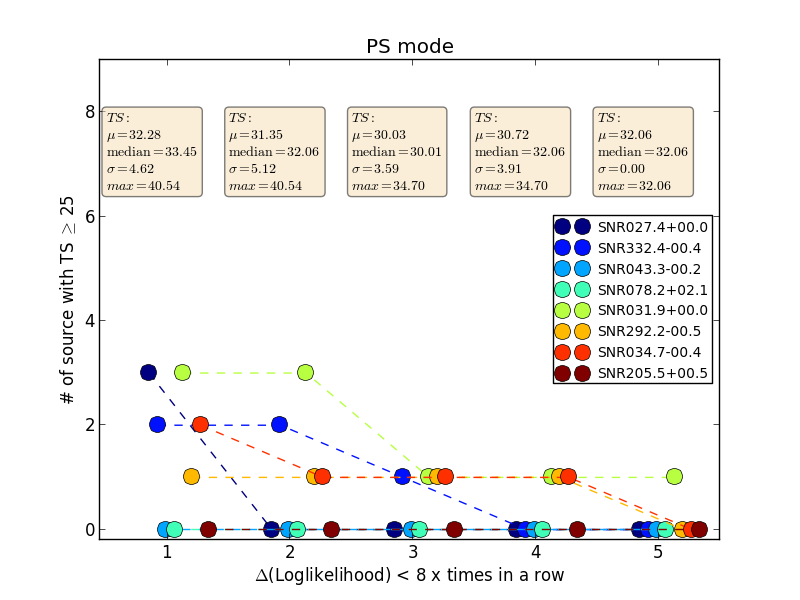
\includegraphics[width=1.0\columnwidth]{Figures/aboveThreshPSgt25.png}}
	\caption[Histogram of the number of significant sources remaining in each of the 8 test RoI for iterations in which $\Delta(\logL) < 8$]{Histogram of the number TS $\geq$ 25 sources remaining in each of the 8 test \roi{} for iterations in which $\Delta(\logL) < 8$ (\ie{} TS $<$ 16). Points are offset for each SNR for clarity. The text boxes detail statistics for the values of TS of significant sources for the 8 studied SNRs for each corresponding value on the x-axis.}
	\label{fig:NTSthresh}
\end{figure}

\begin{figure*}[ht]
	\begin{center}
		\hspace*{-1.5cm} \begin{tabular}{ll}
			\includegraphics[width=8cm]{Figures/{ES_1_Flux_SNR078.2p02.1_ES_noColor}.png} &
			\includegraphics[width=8cm]{Figures/{ES_1_Index_SNR078.2p02.1_ES_noColor}.png} \\
			\multicolumn{2}{c}{\includegraphics[width=8cm]{Figures/{ES_1_Sigma_SNR078.2p02.1_ES_noColor}.png}}\\
		\end{tabular}
	\end{center}
	\caption[SNR Gamma Cygni flux, index, and extension evolution for successive \srcs{} iterations]{
		\label{fig:gamCygEvo}{Flux (upper left), \pl{} spectral index (upper right), and extension (lower panel) evolution of the extended source coincident with \snr{} gamma Cygni (labeled ES 1 in the figures) as successive sources are added to the \roi{}.  Dotted line is first time $\Delta(\logL) < 8$, dashed line shows the final threshold for this test study.}
	}
\end{figure*}


To allow for proper convergence of the likelihood fit, we reduced the number of free parameters prior to each new source addition. If the previously added source was between $3$\degr{} and $5$\degr{} from the center of the RoI, just its normalization was freed, and if greater than $5$\degr{} all its source parameters were fixed.
To avoid having newly added sources overlap with pulsars, we deleted new sources from the RoI if they were within~$0.2$\degr{} of a \g-ray pulsar and refit the pulsar in the $1-100$\,GeV range following the 2PC conventions. 
2PC modeled pulsar spectra as a PL with an exponential cutoff (PLEC),
\begin{equation}
\newcommand{\pfrac}[2]{\left(\frac{#1}{#2}\right)} \frac{dN}{dE} = N_0 \pfrac{E}{E_0}^{-\Gamma} \exp\left(-\frac{E}{E_c}\right)^{b},
\label{eqn:PLEC}
\end{equation}
where \textit{$N_0$} is the normalization factor, \textit{$\Gamma$} is the photon spectral index, \textit{$E_c$} the cutoff energy, and $b$ determines to the sharpness of the cutoff. 2PC assessed the validity of fixing $b$ to $1$ in Equation~\ref{eqn:PLEC} (PLEC1) by repeating the analysis using a PL model, as well as the more general exponentially cut off PL form, allowing the parameter $b$ in Equation~\ref{eqn:PLEC} to vary. For the pulsar spectra in this analysis, we compared the maximum likelihood values for spectral models with and without a cutoff and with and without the value of $b$ being free, via $\mathrm{TS_{cut}} \equiv 2 ($\logL{}$_{\mathrm{PLEC1}}-$\logL{}$_{\mathrm{PL}})$ and $\mathrm{TS}_{b} \equiv 2 ($\logL{}$_{\mathrm{PLEC}}-$\logL{}$_{\mathrm{PLEC1}})$ to determine which to use. If $\mathrm{TS_{cut}} < 9$ is reported for the pulsar in 2PC then a PL model is used. If TS$_{\mathrm cut} \geq 9$, we then check to see if the cutoff energy fit in 2PC lies within the restricted energy range of $1-100$\,GeV used in this work. For pulsars with cutoffs $\geq 1$\,GeV, we then use the PLEC model if TS$_{\mathrm b} \geq 9$, and the PLEC model with cutoff freed otherwise. For those pulsars with cutoffs less than 1 GeV the spectral parameters are fixed to the 2PC values.

To complete the construction of our point source RoI model, we took the output of the previous steps and removed all sources with TS~$< 16$. This final model was then used as the starting model for analyzing candidate SNR emission. In Figure \ref{fig:w44initRoi}, we show a residual TS map of the region around \snr{} W44 as an example of the source configuration in an \roi{} prior to running \srcs{}. Figure \ref{fig:w44finRoi} is a residual \ts{} map of the same region after running \srcs{} to decompose the region into point sources, and Figure \ref{fig:w44finRoi_ES} the result after running \srcs{} in extended source mode.

\begin{figure}[ht!]
	\centering
	\makebox[\linewidth]{\includegraphics[width=1.0\columnwidth]{figures/{PS_00_tsmap_wo2FGL_SNR034.7-00.4_PS}.png}}
	\caption[1-100GeV  residual TS map for SNR W44 before running \srcs{} and with 2FGL sources removed from the inner 3$^\circ$ radius.]{1-100GeV  residual TS map for \snr{} W44 before running \srcs{} and with 2FGL sources removed from the inner 3$^\circ$ radius (yellow circle). Bin size is 0.$2^\circ$/pixel. Magenta circle shows a 5$^\circ$ radius. 2FGL and newly added sources are shown as green crosses.}
	\label{fig:w44initRoi}
\end{figure}

\begin{figure}[ht!]
	\centering
	\makebox[\linewidth]{\includegraphics[width=1.0\columnwidth]{figures/{TSgt16_tsmap_wo2FGL_SNR034.7-00.4_PS}.png}}
	\caption[1-100GeV  residual TS map for SNR W44 after \srcs{} has completed in PS mode.]{1-100GeV  residual TS map for \snr{} W44 after \srcs{} has completed adding point sources. 2FGL sources have been removed from the inner 3$^\circ$ radius (yellow circle), and the bin size is 0.$2^\circ$/pixel. Magenta circle shows a 5$^\circ$ radius. 2FGL and newly added sources are shown as green crosses.}
	\label{fig:w44finRoi}
\end{figure}

\begin{figure}[ht!]
	\centering
	\makebox[\linewidth]{\includegraphics[width=1.0\columnwidth]{figures/{TSgt16_tsmap_wo2FGL_SNR034.7-00.4_ES}.png}}
	\caption[1-100GeV  residual TS map for SNR W44 after \srcs{} has completed in ES mode.]{1-100GeV  residual TS map for \snr{} W44 after \srcs{} has completed adding point and extended sources. 2FGL sources have been removed from the inner 3$^\circ$ radius (yellow circle), and the bin size is 0.$2^\circ$/pixel. Magenta circle shows a 5$^\circ$ radius. 2FGL and newly added sources are shown as green crosses, and green circles are extended sources added to the \roi{}.}
	\label{fig:w44finRoi_ES}
\end{figure}
We conservatively allow sources with TS down to $16$ $(\sim4\,\sigma)$ in order to account for the effects of at least the brightest sub-threshold sources on the parameter fits for the other sources in the model. Furthermore, while the SNR analysis method described in the chapter \ref{snrcat:DetectMethod} is allowed to remove sources, it cannot add them. Thus we start from a set of sources designed to allow the final model to capture all significant emission within the central region. To corroborate our method of systematically adding sources to a region, we compare our RoI source models with those found by the 2FGL approach in Chapter \ref{snrcat:addSrcs2FGL}. 



%%%%%%%%%%%%%%%%%%%%%%%%
%%%%%%%%%%%%%%%%%%%%%%%%

\section{Comparison of Source Models with 2FGL}
\label{snrcat:addSrcs2FGL}
This SNR catalog was constructed using $3$~years of P7 Source class data in the energy range $1-100$\,GeV, whereas 2FGL used $2$\,years of data over the larger energy range $0.1-100$\,GeV. The differences in observing time and energy range resulted in residual, unmodeled emission in some RoIs as well as changes to some 2FGL sources' spectral model, position localization, and detection significance. Here we compare the input source models constructed for this catalog, described in Chapter \ref{snrcat:AddSrcs}, with 2FGL to better understand the \srcs{} method's ability to describe the regions studied. Since we rederive the input source model only within a $3\degr$\,radius of the center of each RoI, we consider sources only inside that radius.

Given the data set differences, in each RoI we expect similar but not identical numbers of sources relative to those in 2FGL.
Figures~\ref{fig:2FGLvAddSrcs} and \ref{fig:2FGLvAddSrcsAssoc} show the numbers of significant (TS\,$\geq 25$) 2FGL sources and derived input model sources (excluding 2FGL identified AGN and pulsars kept in the input model) in individual RoIs as 2D histograms. In Figure~\ref{fig:2FGLvAddSrcs}, the number of sources in the derived input model is typically greater than the number of 2FGL sources that are significant at $1-100$\,GeV. 73 of the 279 RoIs studied contain at least one of the the 12 extended 2FGL sources. Since 2FGL extended sources were removed from the inner $3\degr$ of each RoI, and this region was repopulated with point sources, we can detect multiple point sources inside the extent of any removed extended 2FGL sources. This decomposition of extended sources, combined with the longer data set and different energy range compared to 2FGL, contribute to the high ratio of input model to 2FGL sources in some RoI, which demonstrates the need to rederive the source model. 

\begin{figure}[h!]
	\centering
	\makebox[\linewidth]{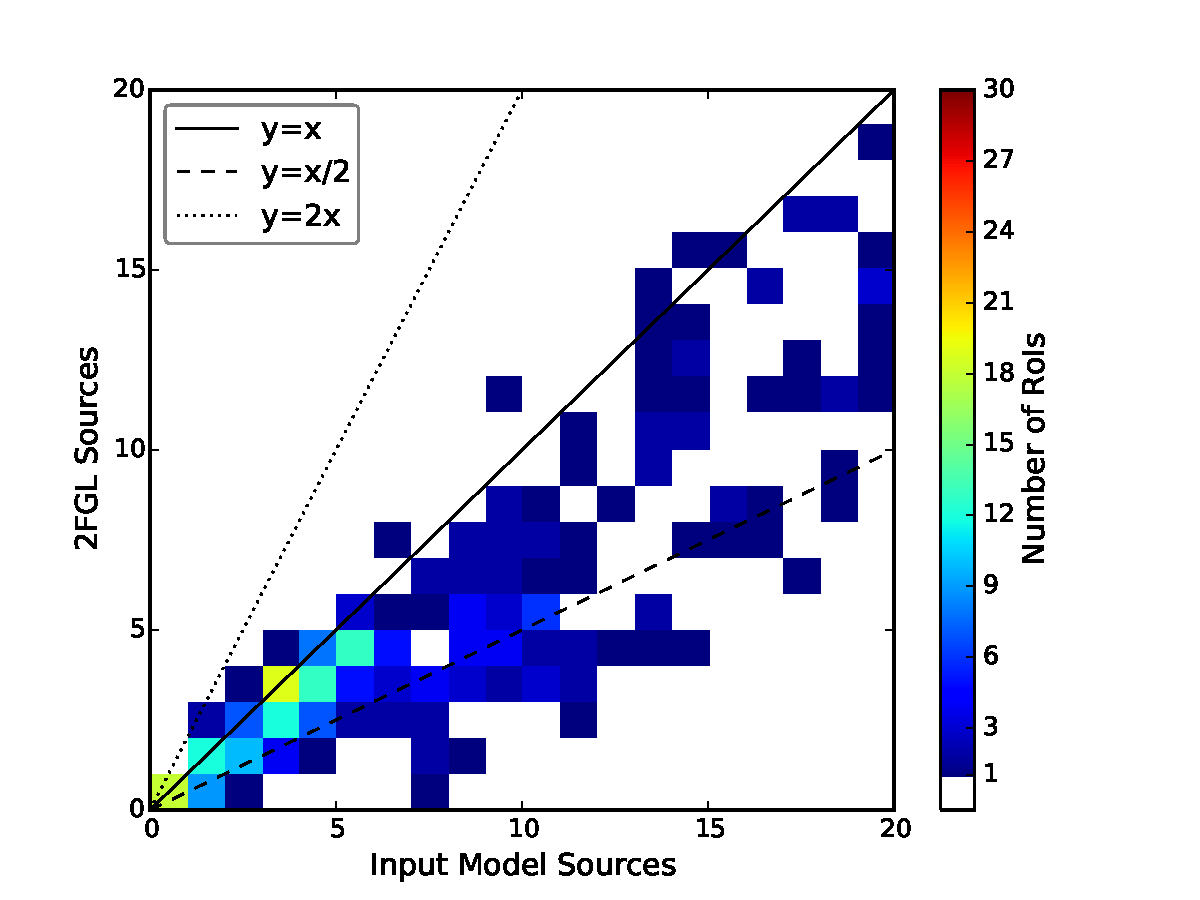
\includegraphics[width=1.0\columnwidth]{figures/addSrcs_2FGLnoAGNPSR_TSgt25_in3deg_2dhist_maj.pdf}}
	\caption[Comparison of the number of 2FGL sources with with the number of newly added input model sources.]{Comparison of the number of 2FGL sources with TS$_{1-100\,\mathrm{GeV}} \geq 25$ (excluding AGN and pulsars) with the number of newly added input model sources in the present analysis, for sources within $3$\degr{} of the center of each RoI. The color scale shows the number of RoIs with a particular combination of numbers of 2FGL sources and new sources. White corresponds to no RoI with that combination of source counts.}
	\label{fig:2FGLvAddSrcs} 
\end{figure}

To more accurately represent the 2FGL sources being reproduced in the central $3\degr$, in Figure~\ref{fig:2FGLvAddSrcsAssoc} we limited the input model sources to those within $0.2\degr$ (approximately the width of the core of the $10$\,GeV PSF) of a 2FGL source, effectively excluding input sources that are not co-spatial with a 2FGL source. Here we see that the majority of 2FGL sources have counterparts in the rederived set. As a region's complexity increases, seen as an increase in numbers of 2FGL sources, up to about half of the 2FGL sources may not have counterparts within $0.2$\degr. Given that in these same regions we have more new sources than 2FGL sources, as seen in Figure~\ref{fig:2FGLvAddSrcs}, we find as expected that the longer data set with improved statistics at higher energies, where the angular resolution of the LAT is the best, allows us to add new sources to account for newly significant excesses in these complex regions. Additionally, sources with low TS in 2FGL are particularly susceptible to having a newly added source which may start at a similar position but then localize further than $0.2\degr$ from the 2FGL source. 

Thus, we find that the method developed and used here produces a model which reproduces the 2FGL sources as expected, including differences that trend as anticipated given the longer data set and modified energy range, yielding better spatial resolution. The new method thus provides reasonable representations of the regions being modeled as input for the final analysis.

\begin{figure}[h!]
	\centering
	\makebox[\linewidth]{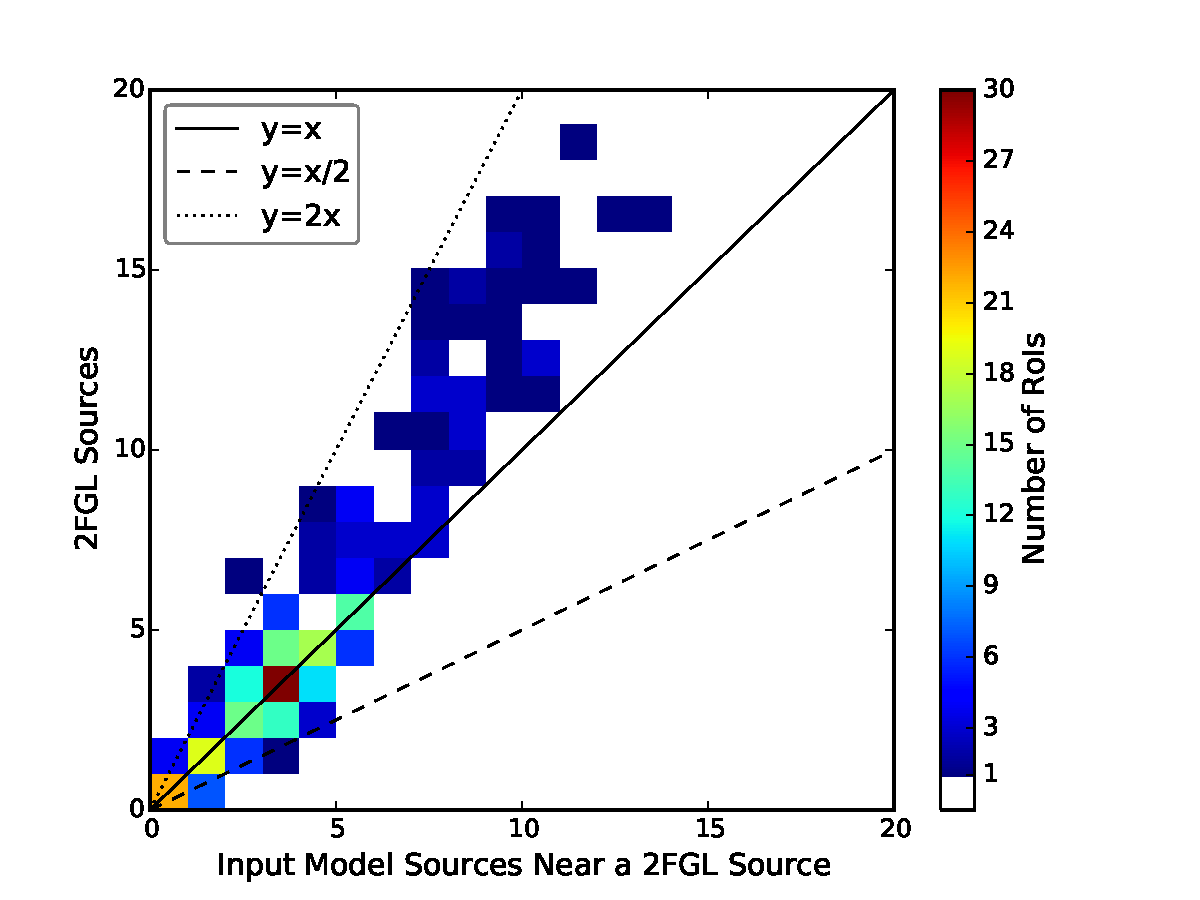
\includegraphics[width=1.0\columnwidth]{Figures/addSrcsWassoc_2FGLnoAGNPSR_TSgt25_in3deg_2dhist_maj.pdf}}
	\caption[Same as Figure~\ref{fig:2FGLvAddSrcs}, including only input model sources lying within $0.2$\degr{} of a 2FGL source.]{Same as Figure~\ref{fig:2FGLvAddSrcs}, including only input model sources lying within $0.2$\degr{} of a 2FGL source.}
	\label{fig:2FGLvAddSrcsAssoc} 
\end{figure}

%%%%%%%%%%%%%%%%%%%%
%  ANALYSIS SECTION
%%%%%%%%%%%%%%%%%%%%

\section{Detection Method}\label{snrcat:DetectMethod}
For each SNR, we characterize the morphology and spectrum of any \gam{} emission that may be coincident with the radio position reported in Green's catalog. This was achieved by testing multiple hypotheses for the spatial distribution of \gam{} emission: a point source and two different algorithms for an extended disk. The best fit was selected based on the global likelihoods of the fitted hypotheses and their numbers of degrees of freedom. The hypothesis with the best global likelihood was then evaluated using a classification algorithm described in \cite{snrCat} to determine whether the radio SNR could be associated with the detected \gam{} emission. 

Spatial coincidence is a necessary but not sufficient criterion to identify a \gam{} source with a known SNR. The detection of spatially extended \gam{} emission increases confidence in an identification, especially if GeV and radio sizes are similar, as has been observed on an individual basis for several extended SNRs \citep[e.g.][]{Lande12}. The LAT has sufficient spatial resolution to detect many Galactic SNRs as extended. Figure~\ref{fig:size_hist_p} shows the distribution of radio diameters from Green's catalog. Vertical dashed lines show the minimum detectable extension for sources with flux and index typical of those observed in this catalog, based on simulations using the P7V6 IRFs~\citep{Lande12}. The minimum detectable extension depends not only on the source's flux and spectrum, but also the flux of the background, which was estimated by scaling the average isotropic background level by factors of 10 and 100 to be comparable to the Galactic plane. As figure~\ref{fig:size_hist_p} illustrates, roughly one third of the known Galactic SNRs may be resolved by the LAT if they are sufficiently bright GeV sources.

\begin{figure}[h!]
	\centering
	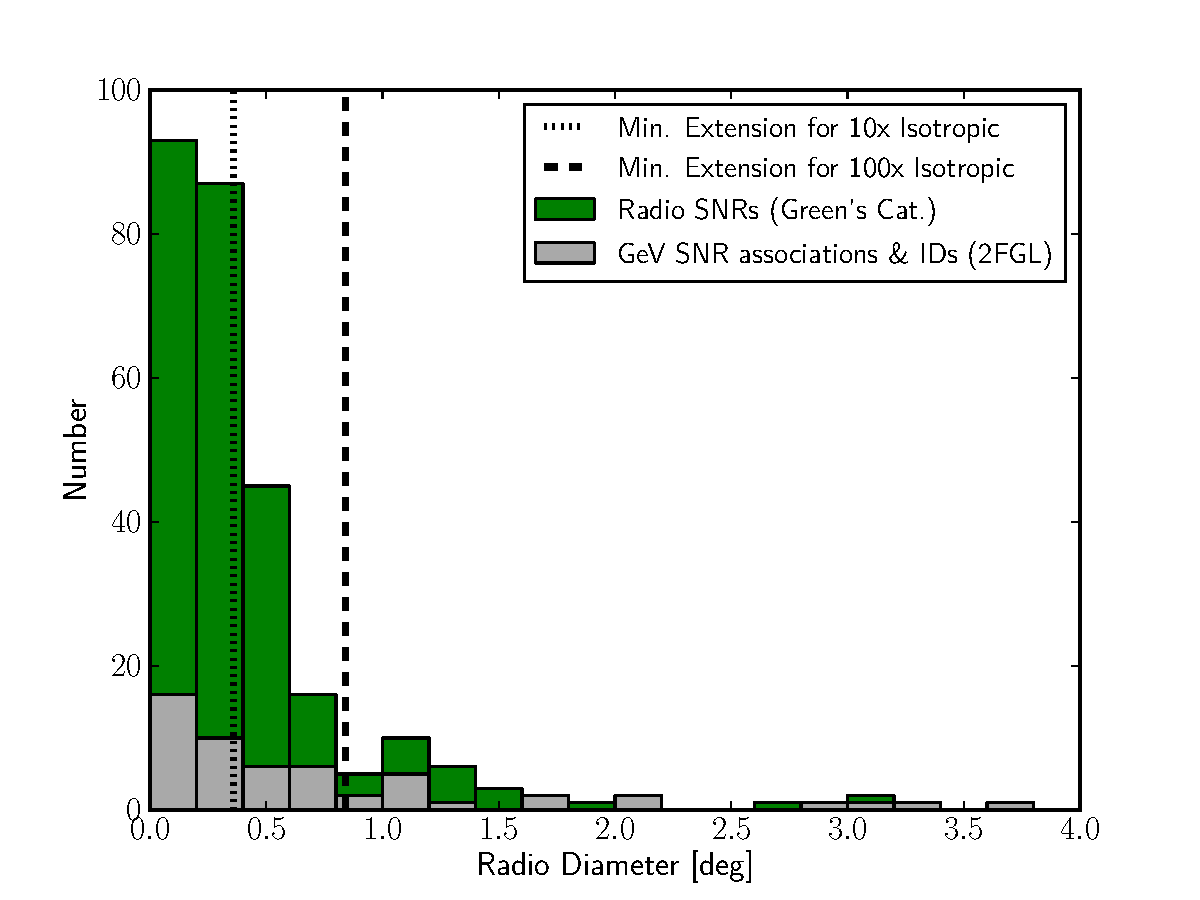
\includegraphics[width=1.0\columnwidth]{figures/size_hist_p.pdf} 
	\caption[Distribution of SNR radio diameters from Green's catalog]{Distribution of SNR radio diameters from Green's catalog. The vertical dashed lines indicate the minimum detectable extension for a source with a photon flux of $10^{-8}$\,ph\,cm$^{-2}$\,s$^{-1}$ in the $1-100$\,GeV energy range and a PL index of $-2.5$, from simulations of $2$\,years of data and the P7V6 IRFs \citep{Lande12}. In that work, simulations using $10$x and $100$x the isotropic background level (thin-dotted and thick-dashed lines) are used to estimate a reasonable background range for sources in the Galactic plane.\jamie{idk what plots are ok or not to include from papers I am an author on. I didnt make this plot, but I made the first version of it that inspired this one. Should I specifically include a comment for these plots that state they're from the snr cat vs ones not in the paper?}}
	\label{fig:size_hist_p}
\end{figure}

In order to determine the best representation for each SNR, we analyzed each SNR-centered RoI using multiple hypotheses for the spatial and spectral form. We used \ptlike{}~\citep{Kerr10} to compare PL and logP spectral forms, to compare point source versus extended source hypotheses, and to analyze the robustness of sources near the extended source.

For each hypothesis, we started with the input model described in Chapters \ref{snrcat:Data} and~\ref{snrcat:AddSrcs}. We removed sources falling within the SNR's radio disk unless they had been identified as an AGN or pulsar, as described in Chapter \ref{snrcat:AddSrcs}. We then proceeded to evaluate the following point and extended source hypotheses. For the point source hypothesis, a point source with a PL index initialized to $2.5$ was placed at the radio centroid of the SNR. The positions, spectral index, and spectral normalization of the point source were then fit. As for the initial input model described in Chapter \ref{snrcat:AddSrcs}, we tested the source for spectral curvature. To test the extended source hypothesis, we employed two separate procedures. Both employed a uniform disk model initially placed at the center of the RoI with a radius equal to that observed in the radio. In the first procedure, called the ``disk" hypothesis, we fit both the position and extension of the disk, as well as tested for spectral curvature. A second procedure, which results in a model we call the ``neardisk" hypothesis, additionally examines the significance of sources nearby the disk, removing those which are not considered independently significant and refitting the disk position and radius. This procedure is described in Chapter \ref{snrcat:LocExtSpec}.

Having evaluated these hypotheses, we compared the global likelihood values of the final extended hypothesis and of the point source hypothesis to determine which model had the largest maximum likelihood. If the source is significant in the best hypothesis, the model parameters are reported as Tables 1 and 2 in \cite{snrCat} \jamie{should I include abridged tables?}. If no hypothesis had a significant \gam{} source coincident with the radio SNR, we calculated the upper limit on the flux from a region consistent with the radio SNR, described in Chapter \ref{snrcat:FluxULs}, and report  the results in Table 3 in \cite{snrCat}. \jamie{should I include the tables here? only if they're short, or abridged. I should def include the dist table because I did that work}

\subsection{Localization, Extension, and Spectral Curvature}\label{snrcat:LocExtSpec}
To test our hypotheses, we combined the initial model of point sources (Chapter \ref{snrcat:AddSrcs}) and the Galactic and isotropic diffuse contributions (Chapter \ref{snrcat:Data} and \ref{snrcat:AddSrcs}) with a test source at the center of each RoI. All sources that fell within the radio SNR radius other than previously identified AGN or pulsars were removed, as was done for the input source model (Chapter \ref{snrcat:AddSrcs}). We note that multiple point sources removed within a single radio SNR radius may represent substructure within the source itself. This process conservatively assigns the majority of the flux to a single source, rather than decomposing it. We optimized the position of the test source with \ptlike{}, iteratively allowing other model parameters to vary. For all hypotheses, the normalizations of all sources within $5$\degr{} of the radio SNR center were fit while all other spectral parameters were fixed. The parameters for sources outside $5$\degr{} were also fixed.

For the point source hypothesis, a point source was placed at the radio centroid of the SNR. For the disk hypothesis, a uniform disk with radius equal to the radio radius was placed at the center. In both hypotheses, the normalization, index, and position of the candidate source were fit. For the disk hypothesis, the extension was also fit. Previous analyses of a range of possible Galactic SNR sources with similar data sets \citep[e.g.][]{Lande12} typically showed no differences in global likelihood significant enough to justify choosing a Gaussian over a uniform disk template or vice versa. In addition, there was typically little difference in spectral parameters for the two spatial forms. For simplicity and clarity, we thus test only the uniform disk hypothesis. We allowed the localization to wander up to  $5$\degr{} in the fits as a reasonable upper limit on what might later be associated with the SNR. This is roughly twice the radius of largest radio SNR.

We included an additional disk hypothesis in which we recalculated the significance of each nearby point source. Because neighboring sources can influence the best fit disk parameters, we iteratively evaluated the significance of the neighboring source by calculating TS$_{\rm nearby}$, defined as twice the difference between the model's log-likelihood (\logL{}) with the nearby point source and the model without the source, as determined by \ptlike. Starting from the fitted disk model, for each neighboring point source we refit the position, extension, normalization, and spectrum of the uniform disk after removing the source. A nearby source was considered to be significant and thus kept if TS$_{\rm nearby} \geq 9$. Each point source was evaluated individually, starting with the closest point source and extending radially outward to all sources within $1$\degr{} of the furthest edge of the SNR's radio disk. The final result of this iterative process is called the ``neardisk" hypothesis which, for cases where neighboring source(s) were removed, can have different best fit disk parameters. As a final step we refit the region with \gtlike, using the neardisk model.

We chose the best extended source hypothesis by comparing the final disk and neardisk \gtlike{} \logL{} values. Since the neardisk hypothesis can have fewer degrees of freedom, we chose the final disk hypothesis only if $2\times$(\logL{}$_{\rm disk}$-\logL{}$_{\rm neardisk}$) $\geq 9$. Otherwise, we used the neardisk model as the final extended source hypothesis, hereafter referred to as the ``disk hypothesis''.

In some cases a point source could not be localized starting at the SNR center. If the \ptlike{} localization failed to converge when starting at the SNR center, we placed the candidate at the position of the most significant source removed from within the radio SNR radius and followed the procedure outlined above. For $69$~RoIs there was either no source removed within the radio SNR or localization failed. For $31$~RoIs, the candidate found had a TS~$<1$ and was removed from the model so as not to cause instabilities in the minimization. If the disk hypotheses converged and the final candidate was significant (TS~$\geq 25$) in both the localization and spectral fits, the best extended hypothesis was selected. 

Prior to the final fit of the region, sources were tested for spectral curvature using $\mathrm{TS_{band fits} - TS_{PL}}\geq~25$. If this criterion was satisfied then we replaced the PL spectral model with a logP model and refit the RoI. The final spectral model was selected, as for the input model, by comparing the \logL{} values, in this case $\mathrm{TS_{curve}} \geq 16$, as defined in Chapter \ref{snrcat:AddSrcs}. Seven sources were found to be significantly better fit by a logP spectrum. To obtain final spectral parameters, we performed a final fit using the standard likelihood analysis tool \gtlike. The normalization and index parameters were constrained to lie within a physically reasonable range. 

%%%%%%%%%%%%%%%%%%%%%%%%%%%%%%%%%%%

We determined the final RoI model by selecting the most likely hypothesis based on a comparison of the \gtlike{} global \logL{} of the point source hypothesis with the most likely extended source hypothesis. An extended hypothesis was considered significantly more likely if $\mathrm{TS_{ext}}$ was $\geq 16$, where $\mathrm{TS_{ext}}$ is defined as twice the difference between the \logL{} of the final model from the disk hypothesis and that of the point source hypothesis, $\mathrm{TS_{ext}} =  2 ($\logL{}$_{\mathrm{disk}}-$\logL{}$_{\mathrm{point}})$, as in~\citet{Lande12}. Otherwise, if the point source itself had TS\,$>25$, we chose the point source hypothesis. In cases in which the optimization for the position of the point source did not converge but an extended disk was detected, we calculated the global \logL{} of the region without any source and with a point source at the center of the extended source. We then use the latter value to calculate $\mathrm{TS_{ext}}$ reported in Table 1 in \cite{snrCat}. For these candidates, if the source was significantly extended in both cases, we select the extended hypothesis. If none of the criteria were met, the candidate was considered undetected and we calculated an upper limit on the flux. Both the upper limits and flux calculation are described in the following subsection.

\subsection{Fluxes and Upper Limits}\label{snrcat:FluxULs}
Fluxes in the $1-100$\,GeV band are determined using the standard analysis tool \gtlike{} by a final fit of the model chosen to have the overall maximum likelihood characterization of the morphology and spectrum of the candidate source from the analysis detailed in Chapter \ref{snrcat:DetectMethod} and \ref{snrcat:LocExtSpec}. For those RoIs where no significant source was detected, we computed Bayesian upper limits on the flux using the method in described in \citet{Helene83} excluding any overlapping sources in the model that have not been identified as AGN or pulsars, as described in Chapter \ref{snrcat:AddSrcs}. As a spatial model we used a uniform disk equal in position and radius to that reported in Green's catalog. We assumed the spectral model to be a PL and report upper limits for indices of $2.0$ and $2.5$ at $95\%$ and $99\%$ confidence levels. The choice of indices was motivated by the distribution of PL indices for classified sources. The results are reported in \cite{snrCat}.

%%%%%%%%%%%%%%%%%%%%%%%%
%%%%%%%%%%%%%%%%%%%%%%%%

\section{Catalog Results}\label{snrcat:TheCatalog}
We detected \ndetected~candidates with a final source TS\,$\geq 25$ in the \nGalSNRs~SNR RoIs (see Chapter \ref{snrcat:DetectMethod}). Of the \ndetected~detected candidates, \nassocprobclassified{} passed the association probability threshold (see \cite{snrCat}). Of these, \nclassifiedsnrs~SNRs ($\sim11\%$ of the total) show significant emission for all alternative IEMs and are classified as likely GeV SNRs. An additional \nnotsnrs{} were identified as sources which are not SNRs.Two other candidates were demoted to marginal due to their dependence on the IEM, as described in the next paragraph. Of the sources likely to be GeV SNRs, \nextended~show evidence for extension (TS${\rm_{ext} > 16}$). Only sources associated with SNRs G34.7$-$0.4 and G189.1+3.0 show evidence of significant spectral curvature in the $1-100$\,GeV range and are fit with logP spectra. Of the classified candidates, \nnewextended~extended and \nnewpointlike~point SNRs are new and published here for the first time. Descriptions of the new extended (G24.7+0.6, G205.5+0.5, G296.5+10.0, and G326.3$-$1.8) \snrs{} is given in \cite{snrCat}.
%We describe the \nnewextended~new extended SNRs, G24.7+0.6, G205.5+0.5, G296.5+10.0, and G326.3$-$1.8, in Section~\ref{snrcat:NewSNRs}. 

For those \nULs~SNRs that are either not detected by this analysis or which fail to meet the most stringent threshold for classification as a detected SNR, upper limits assuming the radio disk morphology of Green's catalog with PL indices of $2.0$ and $2.5$ are reported in Table 3 in \cite{snrCat}. For those candidates which fail to meet the most stringent threshold, we replaced the source with the radio disk. We do not calculate upper limits for the \nnotsnrs~sources which are identified as not SNRs. A FITS version of the catalog is available through the \Fermi{} Science Support Center, as described in \cite{snrCat}\footnote{\url{ http://fermi.gsfc.nasa.gov/ssc/data/access/lat/1st_SNR_catalog/}}. \jamie{not including the detailed description of the new SNRs}

\jamie{all the multiwavelength CR stuff and  I wasn't so involved in, but it's kind of the crux of the paper. I don't know how much of if it, if any to include here.}

%%%JAM COMMENTED OUT THESE TABLES
%\input{t1.tex} %{tables/results_v4_0516_det_spatial.tex}  % reference as \ref{Tab:ResultsSpat}
%\input{t2.tex} %{tables/fluxTable2_v7/results_v4_0516_det_spectral_v7.tex} % reference as \ref{Tab:ResultsSpec}
%\input{t3.tex} %{tables/results_v4_0516_UL.tex}   % reference as \ref{Tab:ResultsULs}

%%%%JAM commented this out for now
%\begin{figure}[h!]
%   \centering
%   \includegraphics[width=0.8\columnwidth]{f9.pdf} %{figures/gev_flux_vs_index.pdf}
%   \caption{
%       The distribution of fitted photon index and flux in the energy range $1-100$\,GeV. The index shown for sources for which the logP form is more significant is determined from re-fitting the sources with a PL spectral form rather than their parabolic index $\alpha$, for consistency. Open circles indicate extended SNRs while filled circles indicate point-like sources. All SNRs that passed classification are shown as black unless also classified as young non-thermal X-ray SNRs (blue) or as interacting with MCs (red). Candidates which did not pass classification but still had both fractional overlaps $>0.1$ are grey. If they are also young or interacting, they are outlined in blue or red, respectively\protect\footnotemark. These classes are further defined in Section~\ref{Sec:GeVSNRDiscussion}. Statistical error bars have caps; error bars without caps represent the systematic error, described in Section~\ref{Sec:SysErr}. 
%       \label{fig:GeVFluxGeVIndex}}
%\end{figure}
%\footnotetext{No extended marginally classified candidates were also identified as young or interacting.} 


%%%%%%%%%%%%%%%%%%%%%%%%
%%%%%%%%%%%%%%%%%%%%%%%%

\section{GeV Supernova Remnants in a Multiwavelength Context: Discussion Summary}\label{snrcat:resSum}
%\emph{Here, we summarize some of the findings detailed in the \snrcat{} that are most pertinent to the work performed for this thesis.} \jamie{do I need a statement like  this?}

As discussed in Chapter \ref{gamAstr:Emiss}, the same population of radio, synchrotron-emitting \cray{} electrons active in the shell of an \snr{} are expected to also produced \gam{}s through the \ic{} process and non-thermal \brems{} radiation. If indeed the\gev{} and radio emission are produced in a single zone, it is reasonable to assume that the radio and \gam{} morphologies will correlate. We find that the best GeV diameter is within errors of the radio diameter for most of the candidates classified as being associated with an SNR, as shown in Figure \ref{fig:GeVradioSize}. The same, co-spatial, electron population producing the\gev{} and radio emission is also suggestive of a potential correlation between the radio and \gam{} flux. Figure \ref{fig:GeVradioFlux} shows the 1 GHz synchrotron flux versus the 1\gev{} \gam{} flux for all \snrs{}. Various factors, such as the lack of detailed non-thermal emission modeling, distance measurement errors, and use of oversimplified \gam{} spectral models can skew these results, obscuring any inherent correlation.

\begin{figure}[h!]
	\centering
	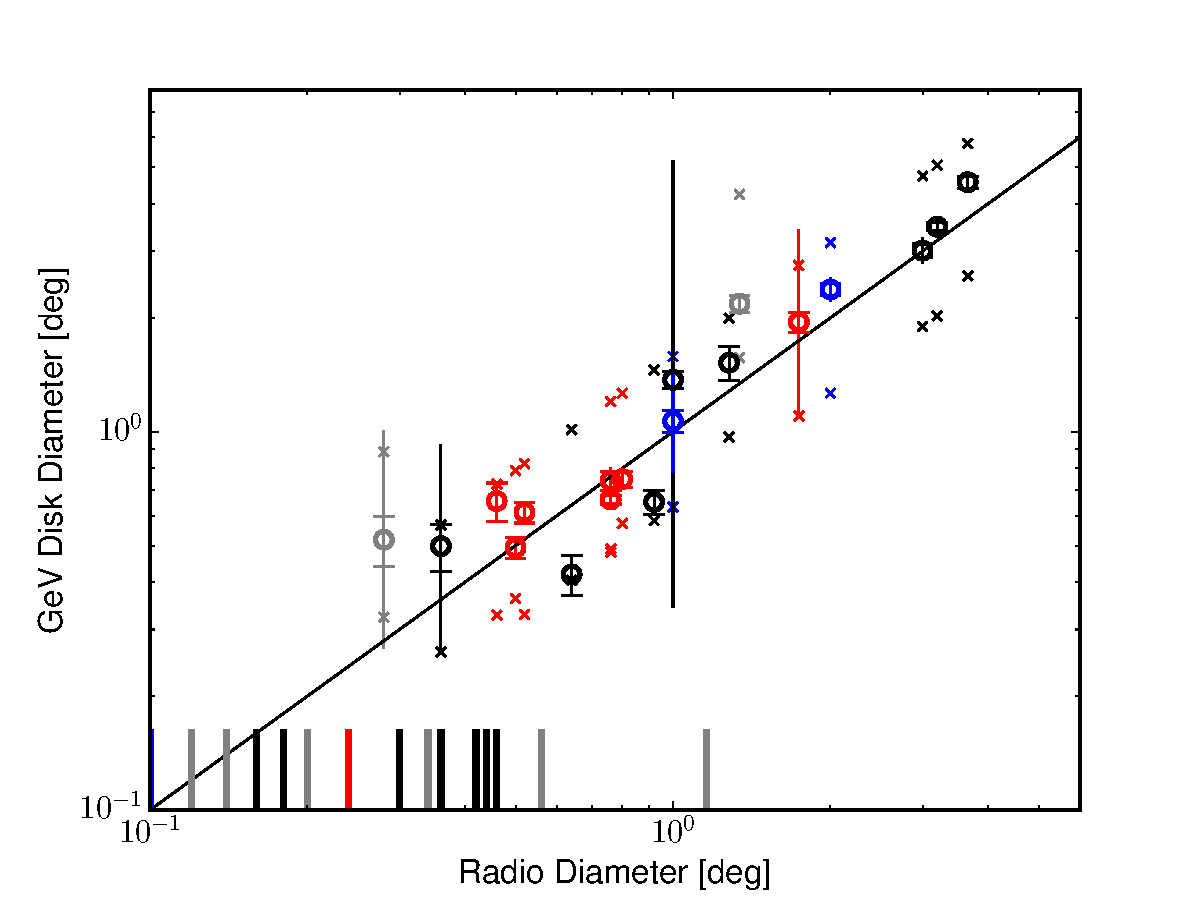
\includegraphics[width=1.\columnwidth]{figures/size_radio_vs_gev_xLims.pdf}
	\caption[Radio diameter of Green's catalog SNRs plotted against the fitted GeV diameter]{Radio diameters of Green's catalog SNRs plotted against the fitted GeV diameters for those candidates with significant extension. The solid line represents equal radio and GeV diameters. All cases of detected extension have diameters greater than $0.2$\degr. The ticks denote the radio extension of GeV point-like candidates, colored in order of their characteristics (young or interacting) and by their classifications (well defined or marginal). The small `x's bracketing the points show the minimum and maximum GeV extensions allowed such that the source remains classified or marginally classified  given the radio position and extension and best fit GeV position. Open circles indicate extended SNRs. All SNRs that passed classification are shown as black unless also classified as young, non-thermal X-ray SNRs (blue) or as interacting with MCs (red). Candidates that did not pass classification but that still had both fractional overlaps $>$ 0.1 are gray.  Statistical error bars have caps; error bars without caps represent the systematic error. \jamie{took out the filled circles and outlined part,  If they are also young or interacting, they are outlined in blue or red, respectively (No extended marginally classified candidates were also identified as young or interacting.)}}
	\label{fig:GeVradioSize}
\end{figure}

\begin{figure}[h!]
	\centering
	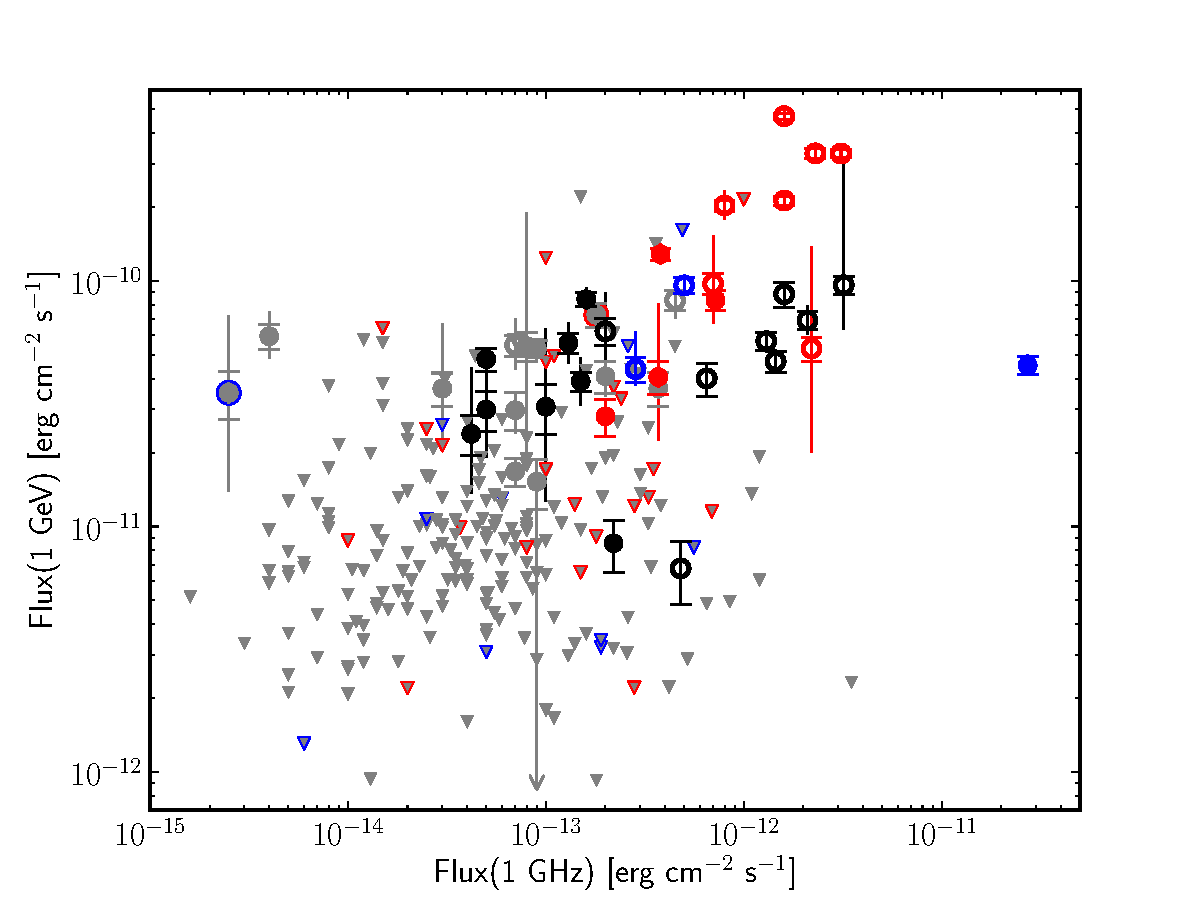
\includegraphics[width=1.\columnwidth]{figures/radio_vs_gamma_nuFnu_flux_ULs.pdf}
	\caption[Comparison of \gam{} and radio spectral flux densities for all SNRs and candidates.]{Comparison of \gam{} and radio spectral flux densities for all SNRs and candidates. For all SNRs that were not detected or which failed classification, grey triangles indicate upper limits at $99\%$ confidence, computed assuming the radio location and extension. Symbols, colors, and error bars are as in Figure \ref{fig:GeVradioSize}. In addition, filled circles indicate point-like sources, and if grey markers are also young or interacting, they are outlined in blue or red, respectively (No extended marginally classified candidates were also identified as young or interacting).
	}
	\label{fig:GeVradioFlux}
\end{figure}

We test for one further relationship between the radio and GeV emission and the underlying particle populations through the measured radio and GeV spectral indices. The energy of synchrotron-emitting leptons traced by $1$\,GHz observations depends on the magnetic field. If radio and GeV emission trace the same underlying particle population, then, at energies below the maximum energy reached by the accelerated particles, the photon indices of radio and \gam{} emission should be correlated. For $\pi^0$ decay and e$^\pm$ bremsstrahlung, the GeV and radio photon indices ($\Gamma$ and $\alpha$ respectively) are related as $\Gamma = 2\alpha + 1$. For IC scattering leptons, the GeV and radio photon indices follow $\Gamma = \alpha + 1$, or in the case in which high-energy leptons have been cooled via synchrotron or IC radiation, $\Gamma = \alpha + 3/2$ \citep{Reynolds08}. Figure \ref{fig:GeVradioIndex} compares the deduced radio spectral index $\alpha$ with the $1-100$\,GeV photon index $\Gamma$. 

\begin{figure}[h!]
	\centering
	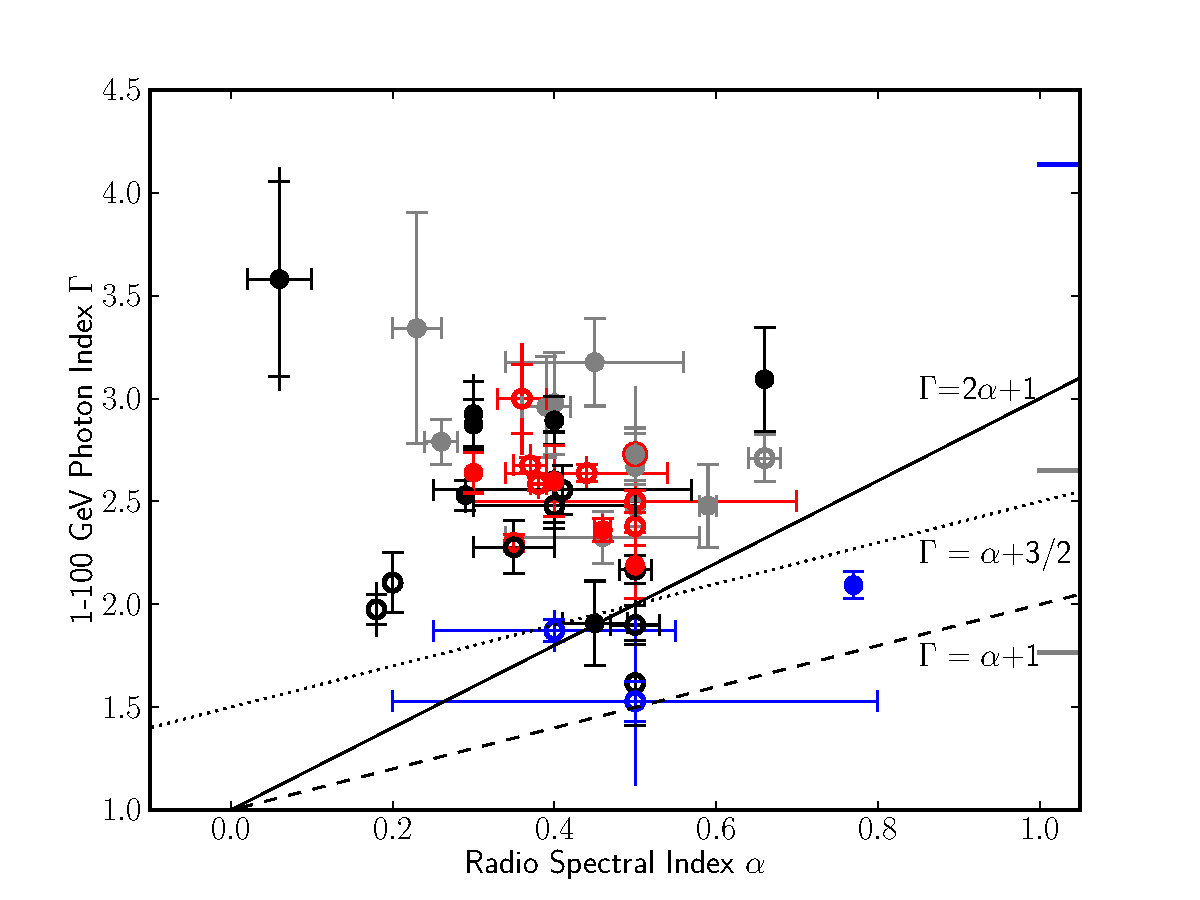
\includegraphics[width=1.0\columnwidth]{figures/radio_vs_gamma_index.pdf}
	\caption[Comparison of radio spectral index, $\alpha$, and GeV photon index, $\Gamma$.]{Comparison of radio spectral index, $\alpha$, and GeV photon index, $\Gamma$. The expected correlations are plotted for $\pi^0$ decay or e$^{\pm}$ bremsstrahlung (solid) and IC emission from an electron population that is freshly accelerated (dashed) or cooled by radiative processes (dotted). Emission via a combination of processes would fall between the lines (e.g. between the solid and dashed for a combination of $\pi^0$ decay and IC emission).  Symbols, colors, and error bars are as in Figure \ref{fig:GeVradioSize}; ticks along the right hand side show the $1-100$\,GeV photon indices of those SNRs without reported radio spectral indices.
	}
	\label{fig:GeVradioIndex}
\end{figure}

Nearly all candidates have \gam{} photon indices that are softer than predicted given their radio spectra, regardless of the GeV emission mechanism. The three young SNRs in blue are most consistent with a single underlying particle population, and it has been suggested they emit via IC (dashed line) at GeV energies. SNRs emitting via a combination of mechanisms under these simple assumptions would have indices falling between the two index relations, that is, they would lie in the region spanned by the $\pi^0$/bremsstrahlung (solid) and IC (dashed) lines. 

The lack of an observed correlation between the indices as expected under these simple assumptions suggests that more detailed physical models are required for the majority of SNR candidates. The observed soft GeV spectra relative to the radio has several potential explanations. 
The underlying leptonic and hadronic populations may have different PL indices. The emitting particle populations may not follow a PL but may instead have breaks or even differing spectral shapes. Finally, there may be different zones with different properties dominating the emission at different wavelengths.

In the \snrcat{}, we also compared the GeV and TeV properties of SNRs to test the second common assumption in SNR models: that momentum distributions of the emitting particle populations do not follow simple PLs but have curvature or breaks. Such changes in spectral slope could also cause breaks in the \gam{} spectra. As TeV emission may originate via the same processes as the \FermiLat-observed GeV emission \citep[e.g.][]{Funk08_GeVTeVGalactic, Tibolla09_HESSUnIds, Tam10_VHEforFermi}, we might expect to see such a change reflected in a spectrum combining \FermiLat{} data with observations from \iacts{} such as \hess{}, \veritas{}, and \magic{}. The converse is also true, where detection predictions in the GeV based on simple PL extrapolation from the TeV have been borne out in GeV studies, e.g. identifications of H.E.S.S. sources from \cite{Tibolla09_HESSUnIds} in 2FGL \citep{2FGL} and \cite{Ackermann12_1FGLUnassoc}. 

In Figure~\ref{fig:GeVTeVIndex} we plot the PL index in the GeV versus TeV range for all SNRs observed with both \FermiLat{} and an IACT detections. Six of the ten SNR candidates have TeV indices that are softer than their GeV indices, while three have GeV and TeV indices that are consistent with each other, within statistical and systematic errors. The remaining interacting candidate has a somewhat softer index at GeV energies than at TeV. Such a hardening of the index from GeV to TeV suggests that another particle population may dominate at higher energies or that the emission mechanism may change between the GeV and TeV regimes. Such curvature in the spectrum may also explain the lack of a simple correlation between GeV and radio PL indices, as described above in this section. We also note that Figure~\ref{fig:GeVTeVIndex} shows a distinct separation between young and interacting SNRs, which are often older. This suggests an evolution in index with age, from harder when younger to softer when older. 

\begin{figure}[h]
	\centering
	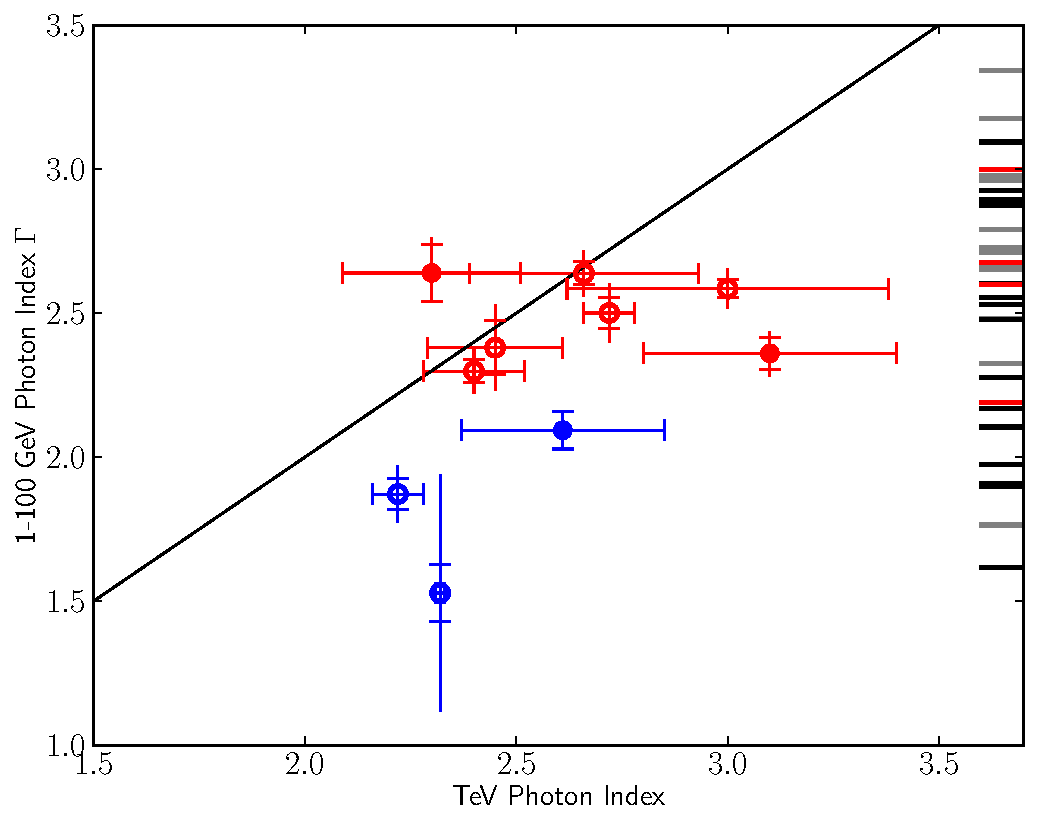
\includegraphics[width=0.8\columnwidth]{Figures/gev_vs_tev_index.pdf}
	\caption[GeV index compared to published index measurements from IACTs.]{GeV index compared to published index measurements from \iacts{}. The line corresponds to equal index values. The predominance of SNRs below the line suggests spectral curvature, potentially reflecting a change in spectral slope of the underlying particle population(s') index or indices. The ticks represent the GeV candidates with indices in the range of those with a TeV counterpart but with no TeV measurements themselves, demonstrating the limitations of the data set. Symbols, colors, and error bars are as in Figure~\ref{fig:GeVradioSize}. 
	}
	\label{fig:GeVTeVIndex}
\end{figure}

In Figure~\ref{fig:AgeGeVIndex}, we take SNR ages from the literature and plot the $1-100$\,GeV photon index versus age. For our uniform sample of all GeV SNR candidates, young SNRs tend to have harder GeV photon indices than interacting SNRs, which are likely middle aged, though the scatter in age for the two classes is one to two orders of magnitude. The general trend of younger SNRs having harder indices may be due to the decrease of the maximum acceleration energy as SNRs age and their shock speeds slow down. This would also result in fewer particles being swept up by the shock front, given a constant density, suggesting a corresponding decrease in luminosity with age.

\begin{figure}[h]
	\centering
	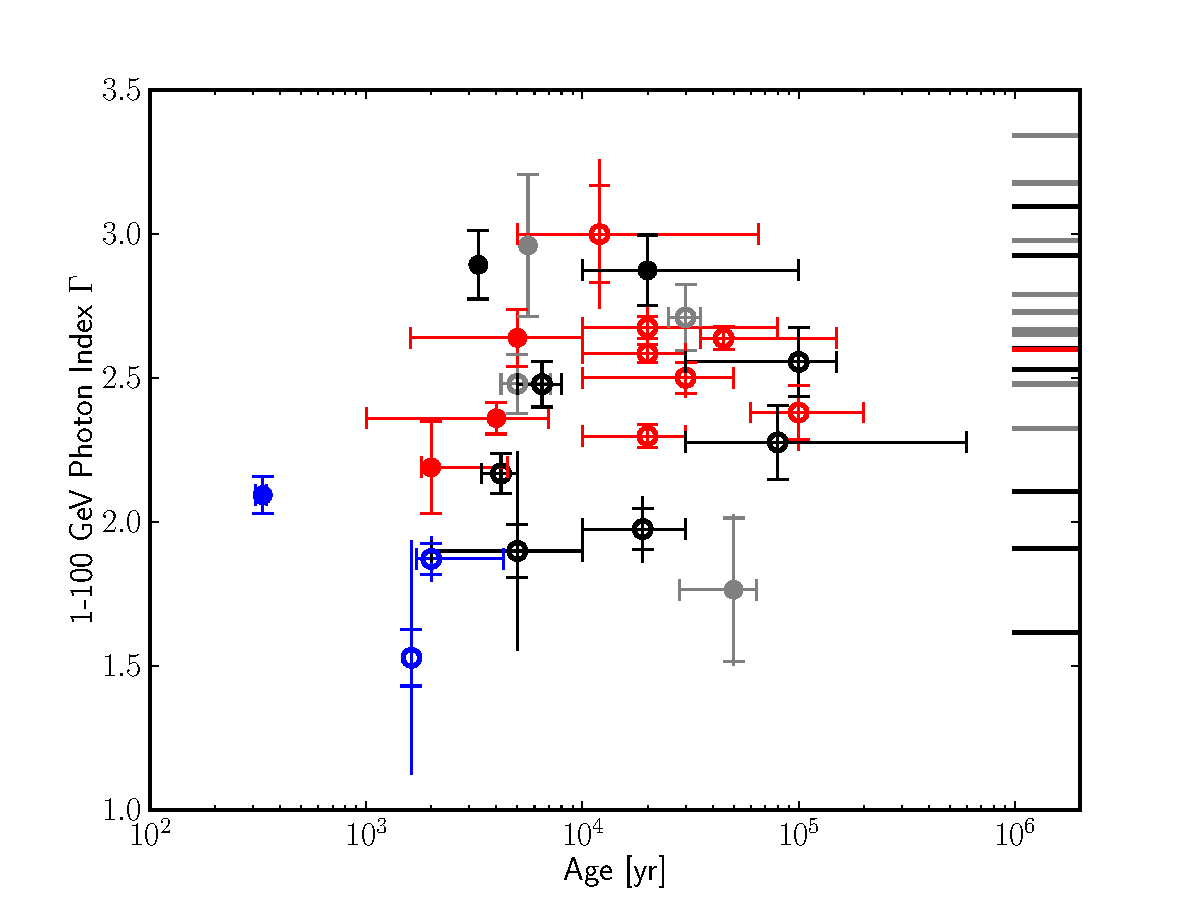
\includegraphics[width=1.0\columnwidth]{Figures/age_vs_index.pdf}
	\caption[Age versus GeV spectral index]{Age versus GeV spectral index. For those with ages in the literature, the young (blue) SNR candidates are separated in this phase space from the identified interacting candidates (red). The ticks on the right show indices for GeV candidates without well-established ages. Symbols, colors, and error bars are as in Figure \ref{fig:GeVradioSize}. 
		\label{fig:AgeGeVIndex}}
\end{figure}

It is important to account for the distances of the SNRs when comparing physical quantities such as luminosity. Table~\ref{Tab:SNRinfo}  records distance from the literature, including the most recent and/or most certain distance estimates adopted in this work. Of the \nGalSNRs~SNRs studied, only \ndist{} have published distance estimates. Most often these distances are determined from observed line-of-sight velocities using an assumed Galactic rotation curve. Furthermore, kinematic distance estimates have largely been done on an individual basis, and are not uniformly determined for all SNRs. We do not consider distances derived using the ``$\Sigma$-D relation" because SNRs show a wide range of physical diameters (D) for a given surface brightness ($\Sigma$), limiting the utility of such a relationship for determining the distances to individual SNRs \citep{Green12-distances}.

\pagestyle{empty}
\begin{deluxetable}{lcll}
	\setlength{\tabcolsep}{0.02in} 
    \tablewidth{0pt}
	\tabletypesize{\scriptsize}
	\tcap{Distances to SNRs \label{Tab:SNRinfo}}
	\tablehead{
		\colhead{Name} & 
		\colhead{d [kpc]} & 
		\colhead{Method} &
		\colhead{Reference(s)}
	}
\startdata
G000.0$+$00.0 & 8.5                           & IAU value & \cite{1986MNRAS.221.1023K} \\
G000.3$+$00.0 & 8.5$^{+3.0}_{-3.0}$          & H\,{\sc i} & \cite{2010ApJS..191..275L} \\
G000.9$+$00.1 & 8.5$^{+7.5}_{-1.5}$          & PSR & \cite{2009ApJ...700L..34C} \\
G001.0$-$00.1 & 8.5                           & Maser & \cite{1999ApJ...527..172Y} \\
G001.4$-$00.1 & 8.5$^{+5.6}_{-0.0}$          & Maser & \cite{1999ApJ...527..172Y} \\
G004.5$+$06.8 & 7.0$^{+2.0}_{-0.6}$          & H\,{\sc i} & \cite{1999AJ....118..926R}, \cite{2005AdSpR..35.1027S}, \cite{2008AA...488..219A} \\
G005.4$-$01.2 & 4.75$^{+0.45}_{-0.45}$       & Maser & \cite{2009ApJ...694L..16H} \\
G005.7$-$00.0 & 8.4$^{+5.3}_{-5.3}$          & Maser & \cite{2009ApJ...694L..16H} \\
G006.4$-$00.1 & 1.9$^{+0.4}_{-0.4}$          & Maser, CO & \cite{2002AJ....124.2145V} \\
G008.7$-$00.1 & 4.5                           & Maser & \cite{1990Natur.343..146K} \\
G009.7$-$00.0 & 4.7                           & Maser & \cite{2009ApJ...694L..16H} \\
G011.2$-$00.3 & 5$^{+21}_{-0.5}$             & H\,{\sc i} & \cite{1972ApJS...24...49R}, \cite{1985ApJ...296..461B}, \cite{1988MNRAS.231..735G} \\
G012.8$-$00.0 & 4.7$^{+1.3}_{-1.1}$          & PSR & \cite{2012ApJ...753L..14H} \\
G013.3$-$01.3 & 3.3$^{+1.8}_{-1.7}$          & CO & \cite{1995ApJ...449..681S}, \cite{1998AJ....116.1323K} \\
G015.1$-$01.6 & 5.7$^{+1.3}_{-3.5}$          & NH & \cite{2008AA...481..705B} \\
G015.4$+$00.1 & 4.8$^{+1.0}_{-1.0}$          & CO & \cite{2013AA...557L..15C} \\
G016.7$+$00.1 & 10.0$^{+3.7}_{-7.4}$         & Maser, CO & \cite{2008ApJ...683..189H}, \cite{2000ApJ...545..874R} \\
G016.8$-$01.1 & 5.1$^{+4.6}_{-1.8}$          & H\,{\sc i} & \cite{2011AA...536A..83S} \\
G018.1$-$00.1 & 5.58$^{+0.24}_{-0.27}$       & H\,{\sc i} & \cite{2014MNRAS.438.1813L} \\
G018.6$-$00.2 & 4.6$^{+0.6}_{-0.6}$          & H\,{\sc i} & \cite{2009AJ....138.1615J} \\
G018.8$+$00.3 & 12.0$^{+3.0}_{-5.1}$         & H\,{\sc i} & \cite{2007AA...474..541T} \\
G021.5$-$00.9 & 4.7$^{+0.4}_{-0.4}$          & PSR & \cite{2006ApJ...637..456C}, \cite{2008MNRAS.391L..54T} \\
G021.8$-$00.6 & 5.35$^{+0.15}_{-0.15}$       & CO, PSR & \cite{2008MNRAS.391L..54T}, \cite{2009ApJ...691..516Z} \\
G023.3$-$00.3 & 4.2$^{+0.3}_{-0.3}$          & H\,{\sc i}, CO & \cite{2008AJ....135..167L}, \cite{2007ApJ...657L..25T} \\
G027.4$+$00.0 & 8.5$^{+0.6}_{-1.0}$          & H\,{\sc i} & \cite{2008ApJ...677..292T} \\
G028.6$-$00.1 & 7.0$^{+1.5}_{-1.0}$          & H\,{\sc i}, NH & \cite{2001PASJ...53L..21B} \\
G028.8$+$01.5 & 4.0                           & NH & \cite{1994AA...286L..47S}, \cite{2010ApJ...725..931M} \\
G029.7$-$00.3 & 7.8$^{+2.8}_{-2.7}$          & H\,{\sc i} & \cite{2008AA...480L..25L} \\
G031.9$+$00.0 & 7.2                           & Maser & \cite{1996AJ....111.1651F} \\
G032.4$+$00.1 & 17                            & NH & \cite{2004PASJ...56.1059Y} \\
G032.8$-$00.1 & 5.2$^{+1.5}_{-0.4}$          & Maser & \cite{2011ApJ...743....4Z} \\
G033.6$+$00.1 & 7.0$^{+1.0}_{-0.5}$          & H\,{\sc i} & \cite{2009AA...507..841G}, \cite{1989ApJ...336..854F} \\
G034.7$-$00.4 & 3.0                           & Maser & \cite{2009AA...498..445P} \\
G035.6$-$00.4 & 3.6$^{+0.4}_{-0.4}$          & H\,{\sc i} & \cite{2013ApJ...775...95Z} \\
G039.2$-$00.3 & 6.5$^{+6.0}_{-0.3}$          & CO & \cite{2009ApJ...694.1266H}, \cite{2011ApJ...727...43S} \\
G041.1$-$00.3 & 10.3$^{+2.5}_{-3.9}$         & CO & \cite{2010ApJ...712.1147J} \\
G043.3$-$00.2 & 10$^{+2}_{-2}$               & H\,{\sc i} & \cite{2001ApJ...550..799B} \\
G049.2$-$00.7 & 4.3$^{+1.7}_{-0.0}$          & Maser, H\,{\sc i} & \cite{1997ApJ...475..194K}, \cite{2009ApJ...706L.270H}, \cite{2013ApJ...769L..17T} \\
G054.1$+$00.3 & 7$^{+2.0}_{-2.5}$            & H\,{\sc i} & \cite{2008AJ....136.1477L} \\
G054.4$-$00.3 & 3.0$^{+0.8}_{-0.8}$          & CO & \cite{1992AAS...96....1J}, \cite{1985AJ.....90.1224C} \\
G069.0$+$02.7 & 1.5$^{+0.6}_{-0.4}$          & H\,{\sc i}, PSR & \cite{2012MNRAS.423..718L} \\
G073.9$+$00.9 & 1.3$^{+0.7}_{-0.8}$          & NH & \cite{1993ARep...37..240L} \\
G074.0$-$08.5 & 0.58$^{+0.06}_{-0.06}$       & PM & \cite{2009ApJ...692..335B} \\
G074.9$+$01.2 & 6.1$^{+0.9}_{-0.9}$          & H\,{\sc i} & \cite{2003ApJ...588..852K} \\
G076.9$+$01.0 & 10.0$^{+5.0}_{-4.0}$         & NH & \cite{2011ApJ...739...39A} \\
G078.2$+$02.1 & 2$^{+2.0}_{-1.5}$            & H\,{\sc i} & \cite{2013MNRAS.436..968L}, \cite{2008AA...490..197L} \\
G089.0$+$04.7 & 1.7$^{+1.3}_{-1.0}$          & CO & \cite{2006ApJ...637..283B} \\
G106.3$+$02.7 & 0.8$^{+1.2}_{-0.1}$          & H\,{\sc i} & \cite{2001ApJ...560..236K} \\
G109.1$-$01.0 & 3.2$^{+0.2}_{-0.2}$          & H\,{\sc i}, CO & \cite{2012ApJ...746L...4K} \\
G111.7$-$02.1 & 3.4$^{+0.3}_{-0.1}$          & PM & \cite{1995ApJ...440..706R} \\
G114.3$+$00.3 & 1.0$^{+1.5}_{-0.3}$          & H\,{\sc i} & \cite{2004ApJ...616..247Y} \\
G116.5$+$01.1 & 1.6                           & H\,{\sc i} & \cite{2004ApJ...616..247Y} \\
G116.9$+$00.2 & 1.6$^{+1.9}_{-0.0}$          & H\,{\sc i} & \cite{2004ApJ...616..247Y}, \cite{1994ApJ...434..635H} \\
G119.5$+$10.2 & 1.4$^{+0.3}_{-0.3}$          & H\,{\sc i} & \cite{1993AJ....105.1060P} \\
G120.1$+$01.4 & 3.0$^{+2.0}_{-0.6}$          & H\,{\sc i} & \cite{2011ApJ...729L..15T}, \cite{2010ApJ...725..894H}, \cite{2008Natur.456..617K} \\
G127.1$+$00.5 & 1.15$^{+0.35}_{-0.25}$       & H\,{\sc i} & \cite{1977AA....59L..13P}, \cite{1993AA...270..393X}, \cite{2006AA...451..251L} \\
G132.7$+$01.3 & 2.2$^{+0.2}_{-0.2}$          & H\,{\sc i} & \cite{1991AA...247..529R} \\
G156.2$+$05.7 & 1.1$^{+1.9}_{-0.8}$          & NH & \cite{1991AA...246L..28P}, \cite{2007MNRAS.376..929G} \\
G160.9$+$02.6 & 0.8$^{+3.2}_{-0.4}$          & H\,{\sc i} & \cite{2007AA...461.1013L}, \cite{1991AJ....101.1033L} \\
G166.0$+$04.3 & 4.5$^{+1.5}_{-1.5}$          & H\,{\sc i} & \cite{1989MNRAS.237..277L} \\
G180.0$-$01.7 & 1.3$^{+0.22}_{-0.16}$        & PSR & \cite{2004AA...426..555S}, \cite{2007ApJ...654..487N}, \cite{2009ApJ...698..250C} \\
G184.6$-$05.8 & 1.93$^{+0.57}_{-0.43}$       & PM & \cite{1973PASP...85..579T} \\
G189.1$+$03.0 & 1.5                           & Maser & \cite{2006ApJ...652.1288H} \\
G205.5$+$00.5 & 1.5$^{+0.1}_{-0.7}$          & H\,{\sc i} & \cite{1986ApJ...301..813O}, \cite{1985ApJ...292...29F}, \cite{2012AA...545A..86X} \\
G260.4$-$03.4 & 2.2$^{+0.3}_{-0.2}$          & H\,{\sc i} & \cite{1988AAS...75..363D}, \cite{2008AA...480..439P} \\
G263.9$-$03.3 & 0.287$^{+0.017}_{-0.021}$    & PSR & \cite{2001PASJ...53.1025M}, \cite{2001ApJ...561..930C}, \cite{2003ApJ...596.1137D} \\
G266.2$-$01.2 & 0.75$^{+0.15}_{-0.25}$       & PM & \cite{2008ApJ...678L..35K} \\
G272.2$-$03.2 & 4.0$^{+1.0}_{-2.2}$          & NH & \cite{2011ApJ...732..114L} \\
G284.3$-$01.8 & 3                             & CO & \cite{1986ApJ...309..667R} \\
G290.1$-$00.8 & 7$^{+4.0}_{-3.5}$            & H\,{\sc i} & \cite{1996AA...315..243R}, \cite{2002ApJ...564..284S}, \cite{2006MNRAS.369..416R} \\
G291.0$-$00.1 & 5$^{+1}_{-1.5}$              & NH & \cite{1998ApJ...499..273H} \\
G292.0$+$01.8 & 6.2$^{+0.9}_{-0.9}$          & H\,{\sc i}, PSR & \cite{2003ApJ...594..326G} \\
G292.2$-$00.5 & 8.4$^{+0.4}_{-0.4}$          & PSR & \cite{2004MNRAS.352.1405C}, \cite{2000ApJ...541..367C} \\
G296.5$+$10.0 & 2.1$^{+1.8}_{-0.9}$          & H\,{\sc i} & \cite{2000AJ....119..281G} \\
G304.6$+$00.1 & 9.7$^{+4.3}_{-1.7}$          & H\,{\sc i} & \cite{1975AA....45..239C} \\
G308.4$-$01.4 & 9.8$^{+0.0}_{-3.9}$          & NH & \cite{2012AA...544A...7P} \\
G309.2$-$00.6 & 4.0$^{+1.4}_{-2.0}$          & NH & \cite{2001ApJ...548..258R} \\
G315.1$+$02.7 & 1.7$^{+3.7}_{-0.3}$          & PM & \cite{2007MNRAS.374.1441S} \\
G315.4$-$02.3 & 2.5$^{+0.3}_{-0.2}$          & PM & \cite{1996AA...315..243R}, \cite{2003AA...407..249S} \\
G315.9$-$00.0 & 8$^{+2}_{-2}$                & PSR & \cite{2009ApJ...703L..55C} \\
G316.3$-$00.0 & 7.2$^{+22.8}_{-2.5}$         & H\,{\sc i} & \cite{1975AA....45..239C} \\
G318.2$+$00.1 & 4.0$^{+5.4}_{-0.7}$          & H\,{\sc i} & \cite{2011arXiv1104.5119H} \\
G320.4$-$01.2 & 5.2$^{+1.4}_{-1.4}$          & H\,{\sc i}, NH & \cite{1999MNRAS.305..724G} \\
G321.9$-$00.3 & 6$^{+4.0}_{-0.5}$            & H\,{\sc i} & \cite{1993MNRAS.261..593S} \\
G326.3$-$01.8 & 4.1$^{+0.7}_{-0.7}$          & NH & \cite{1996AA...315..243R}, \cite{1993ApJ...419..733K} \\
G327.1$-$01.1 & 6.5$^{+6.5}_{-1.5}$          & NH & \cite{1999ApJ...511..274S} \\
G327.4$+$00.4 & 4.3                           & H\,{\sc i} & \cite{2001ApJ...551..394M} \\
G327.6$+$14.6 & 2$^{+0.2}_{-0.4}$            & PM & \cite{2013Sci...340...45N} \\
G328.4$+$00.2 & 17.4$^{+2.6}_{-5.4}$         & H\,{\sc i} & \cite{2001ApJ...551..394M} \\
G330.2$+$01.0 & 4.9                           & H\,{\sc i} & \cite{2001ApJ...551..394M} \\
G332.4$-$00.4 & 3.3                           & H\,{\sc i}, CO & \cite{2006PASA...23...69P}, \cite{2004PASA...21...82R} \\
G332.4$+$00.1 & 7.5$^{+3.5}_{-4.2}$          & NH & \cite{2004ApJ...604..693V} \\
G335.2$+$00.1 & 1.8                           & CO & \cite{2011AA...526A..82E} \\
G337.0$-$00.1 & 11.0                          & Maser & \cite{1996AJ....111.1651F} \\
G337.2$+$00.1 & 14.0$^{+16.0}_{-0.5}$        & H\,{\sc i}, NH & \cite{2005AA...431L...9C}, \cite{2006ApJ...653L..41C} \\
G337.2$-$00.7 & 5.8$^{+3.8}_{-3.8}$          & H\,{\sc i} & \cite{2006ApJ...646..982R}, \cite{2011ApJ...732..114L} \\
G337.8$-$00.1 & 12.3                          & Maser & \cite{1996AJ....111.1651F} \\
G338.3$-$00.0 & 10.0$^{+3.0}_{-2.0}$         & H\,{\sc i} & \cite{2009ApJ...706.1269L} \\
G343.0$-$06.0 & 1.0$^{+0.5}_{-0.5}$          & H\,{\sc i}, NH & \cite{2010ApJ...709..823K}, \cite{2003AA...403..605W}, \cite{2001MNRAS.325..287W} \\
G346.6$-$00.2 & 11.0                          & Maser & \cite{1996AJ....111.1651F} \\
G347.3$-$00.5 & 1.0$^{+0.3}_{-0.2}$          & H\,{\sc i}, CO & \cite{2005ApJ...631..947M} \\
G348.5$+$00.1 & 9$^{+0.5}_{-2.7}$            & H\,{\sc i} & \cite{2012MNRAS.421.2593T} \\
G348.5$-$00.0 & 6.3$^{+7.4}_{-3.3}$          & Maser & \cite{2012MNRAS.421.2593T} \\
G348.7$+$00.3 & 13.2                          & H\,{\sc i} & \cite{2012MNRAS.421.2593T} \\
G349.7$+$00.2 & 11.5$^{+0.7}_{-0.7}$         & Maser & \cite{1996AJ....111.1651F}, \cite{2014ApJ...783L...2T} \\
G350.1$-$00.3 & 4.5$^{+6.2}_{-0.5}$          & H\,{\sc i} & \cite{2008ApJ...680L..37G} \\
G351.7$+$00.8 & 13.2$^{+0.5}_{-11.1}$        & H\,{\sc i} & \cite{2007MNRAS.378.1283T} \\
G352.7$-$00.1 & 7.5$^{+0.9}_{-0.7}$          & H\,{\sc i}, CO & \cite{2009AA...507..841G} \\
G353.6$-$00.7 & 3.2$^{+0.8}_{-0.8}$          & H\,{\sc i}, CO & \cite{2008ApJ...679L..85T} \\
G357.7$+$00.3 & 6.9                           & Maser & \cite{1996AJ....111.1651F} \\
G357.7$-$00.1 & 12                            & Maser & \cite{1996AJ....111.1651F}, \cite{2003ApJ...594L..35G}, \cite{2004MNRAS.354..393L} \\
G359.1$-$00.5 & 4.6                           & Maser & \cite{2007IAUS..242..366Y}, \cite{2008ApJ...683..189H} \\
\enddata
\tablecomments{Table of SNR distances drawn from the literature. The method for determining the distance is noted as: CO = line-of-sight velocity from molecular CO lines; H\,{\sc i} = kinematic distance from H\,{\sc i} absorption; NH = extinction estimate from optical or X-rays; Maser = kinematic distance from OH maser velocity; PM = Proper motions; PSR = association with pulsar. The d$_{\rm error}$ values indicate the range of uncertainties from the quoted distance values as assessed in the cited publications. The distance uncertainties are often asymmetric.
}
\end{deluxetable}


To investigate the role of environment in the trends for the young and interacting SNRs, we examined the GeV luminosity versus radio diameter in Figure~\ref{fig:LumDia}. The square of the physical diameter ($D$) can be regarded as a reasonable indicator for SNR age and environment (see \ref{Rems:evo}), as its evolution during the Sedov-Taylor phase follows
\begin{equation}
\label{eq:Sedov}
{\it D} \propto n_0^{-1/5} \ {\it E}_{\mathrm{SN}}^{1/5} \ {\it t}^{2/5}
\end{equation}
where $n_0$ is the ambient density of the surrounding medium, $E_{\mathrm{SN}}$ is the supernova energy, and $t$ is the age of the SNR \citep{1950RSPSA.201..159T,1959sdmm.book.....S}. We can thus use the physical diameter as an age proxy: ``effective age". Any apparent correlation between the luminosity and $D^2$ may be due to their inherent dependence on distance (squared). As observed in earlier works, e.g.~\cite{Thompson12-FermiCRsReview}, Figure~\ref{fig:LumDia} shows that, for the detected candidates, interacting SNRs are generally more luminous for a given physical diameter than young SNRs, though there is large scatter. This suggests that SNRs at the same effective age may be more luminous because they have encountered denser gas ($n_0$). It should also be noted that there is an explicit correlation between the luminosity and physical diameter plotted in Figure~\ref{fig:LumDia} as both are proportional to distance (squared), which is only reliably measured for a subset of our sample. Observational biases, including that young, often smaller and fainter SNRs tend to be more difficult to detect in the radio as well as in \gam{}, may also affect the observed trends.


\begin{figure}[h]
	\centering
	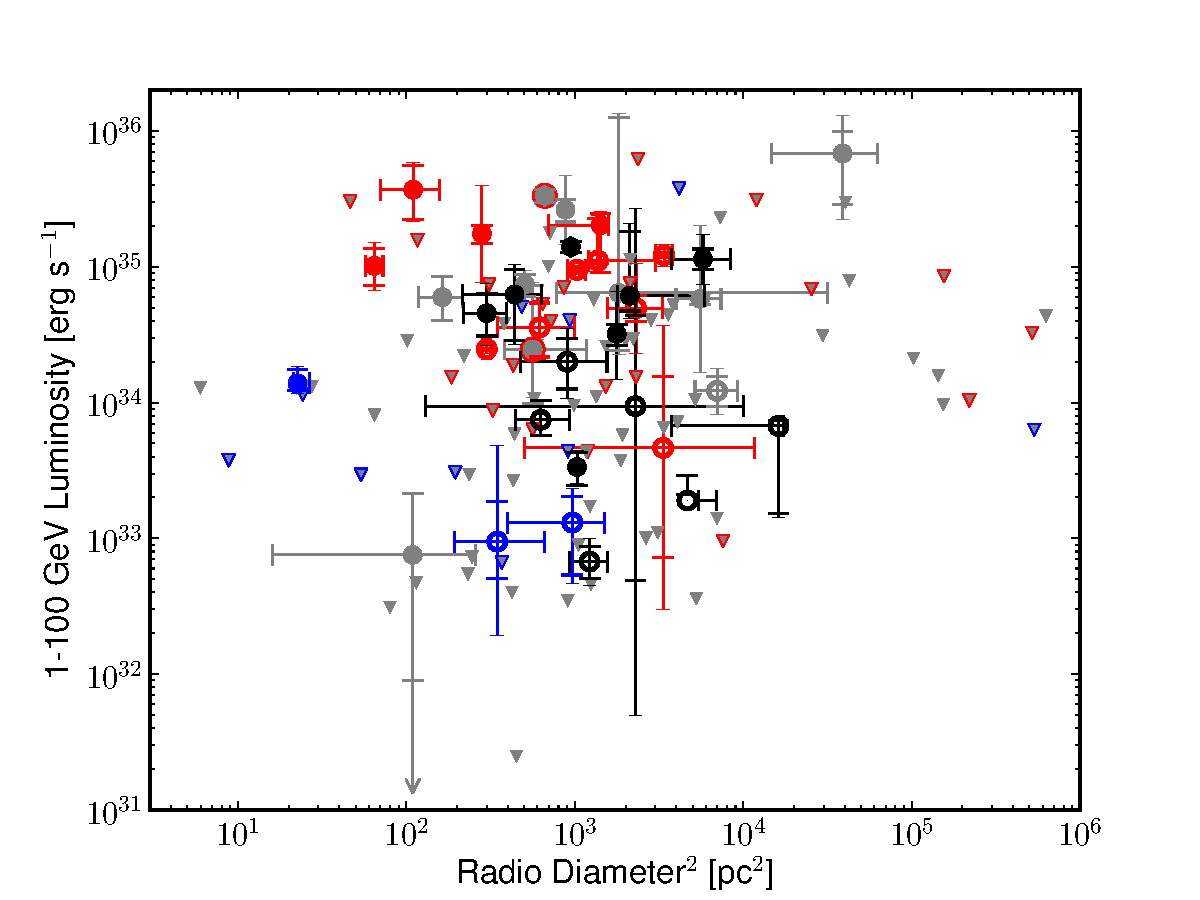
\includegraphics[width=1.0\columnwidth]{figures/lum_vs_dia2.pdf}
	\caption[$1-100$\,GeV luminosity vs. D$^2$ for SNRs with distance measurement.]{
		The $1-100$\,GeV luminosity is plotted against the square of the radio diameters in pc of those SNRs with known distances. Symbols, colors, and error bars are as in Figure~\ref{fig:GeVradioSize}.}
		\label{fig:LumDia}
\end{figure}

\jamie{didn't add anything about maximal CR energy content of all SNRs assuming purely hadronic emission, maybe don't need to}
\section{Conclusions}\label{snrcat:Conclusions}
In this Chapter, we have discussed the state of \gam{} observations of \snrs{} prior to the launch of \Fermi{}, and the unique role that the \lat{} plays in identifying \snrs{} and exploring \gam{} production mechanisms therein. We presented the new automated source addition and analysis method, \srcs{}, and its application to studying the population of \snrs{} emitting\gev{} \gam{}s, published in \cite{snrCat}. With this first \FermiLat{} SNR Catalog we have systematically characterized GeV emission in regions containing known radio SNRs, creating new methods to address issues associated with these typically complex regions. These include methods for systematically adding sources to a region and better estimating the systematic error due to choice of interstellar emission model (discussed in detail in \cite{snrCat}). From this, we have determined characteristics of the GeV SNR population, down to our measurement limit, finding \nclassifiedsnrs~classified and \nmarginal~marginal candidates with a false identification limit of $< $\nninetyfivemockpercent  \citep{snrCat}. This GeV data provide a crucial context for the detailed modeling of individual SNRs. In combination with multiwavelength measurements, the GeV data now challenge simple, previously sufficient SNR emission models. Within the limits of existing multiwavelength data, our observations generally support previous findings of changes in spectral slope at or near TeV energies and a softening and brightening in the GeV range with age and effective age, yet we see indications that new candidates and new multiwavelength data may provide evidence of exceptions to this trend. % With uniformly measured data for all known SNRs, we also constrain SNRs' aggregate, maximal contribution to the population of Galactic CRs. With the GeV and other multiwavelength data, we find that the candidates and upper limits are generally within expectations if SNRs provide the majority of Galactic CRs and anticipate these limits will improve with both a larger GeV data set with better sensitivity, as will be provided by \FermiLat~Pass 8 data, and with more and better distance and density estimates.



